%%% Local Variables:
%%% mode: latex
%%% TeX-master: t
%%% End:
% !Mode:: "TeX:UTF-8"

\documentclass[master]{bnuthesis}
% \documentclass[%
%   bachelor|master|doctor, % mandatory option
%   xetex|pdftex|dvips|dvipdfm, % optional
%   twoside,  % 是否双面打印,默认为单面
%   secret,  % 是否涉密
%   arialtoc,arialtitle]{bnuthesis}

% 所有其它可能用到的包都统一放在这里,可以根据实际需要添加或者删除。
\usepackage{bnutils}
\usepackage{graphicx,multirow}
\usepackage{gensymb}

% 你可以在这里修改配置文件中的定义,导言区可以使用中文。
% \def\myname{薛瑞尼}

\begin{document}

% 定义所有的eps文件在 figures 子目录下
\graphicspath{{figures/}}

%%% 封面部分
\frontmatter
% !Mode:: "TeX:UTF-8"

%%% Local Variables:
%%% mode: latex
%%% TeX-master: t
%%% End:
%\secretlevel{绝密} \secretyear{10}

\ctitle{多核芯片的温敏低功耗调度研究}
%\makeatletter
\cdegree{硕士}

\makeatother

\cauthor{闫佳琪}
\csupervisor{骆祖莹\;副教授}
\cdepartment[]{信息科学与技术学院}
\cmajor{通信与信息系统}
\cnum{201121210009}
\cdate{\the\year  年 \the\month  月}

\etitle{On Temperature and Power Management for MPSoC}

% 定义中英文摘要和关键字
\begin{cabstract}

当前,面向复杂应用的高性能片上系统为了规避和减轻功耗墙问题,延续摩尔定律, 采用了实时温度功耗管理与多核并行计算结构两种主要的技术手段。

% CJC paper abstract

实时功耗温度管理(DPTM)通过对任务的准确预测与合理调度,可以有效地降低片上系统的运行能耗与峰值温度。 为了获得更好的DPTM调度效果,本文在第一部分提出了一种精确的组合式任务预测算法,一种任务调度算法VP-TALK, 进而构建了一个完整的DPTM原型系统。 为了对复杂任务进行精确地任务预测,本文DPTM系统先将复杂任务按频谱长短分类为随机/周期/趋势等三种成分, 然后采用灰色模型/傅里叶模型/径向基函数(RBF)神经网络模型对这三种成分进行组合分析, 以获得精确的预测效果;基于精确预测的任务负载量, 本文所提出的VP-TALK算法可以计算出最优电压-频率对的理想值, 进而选择出两组与理想值相邻的电压-频率对、以获得两个现实的工作状态, 并考虑核心温度和任务实时性的条件,VP-TALK算法将任务负载分配到这两个工作状态, 以获得最优的DPTM效果;最后基于机器学习方法,我们综合四种源算法、构建了一套完整的DPTM原型系统。

实验结果表明:
本文系统的任务预测组合方法的平均误差仅为2.89\%;
在相同的设定峰值温度约束下,与已有调度算法的能耗值相比,尽管假设了更为敏感的功率-温度影响关系, 但对于较高的工作负载率,本文所提出的VP-TALK调度算法仍能够获得平均14.33\%的能耗降低;
本文所提出DPTM原型系统可以获得接近于理想的能耗优化效果;


多核片上系统(MPSoC)的低功耗设计与实时功耗温度管理(DPTM)是目前重要的研究问题。 本文采用了自下而上的建模方法对MPSoC结构级热分析方法进行了研究,提出了三种具有不同算法复杂度与精度的热分析方法: 模块级方法BloTAM、核级方法CorTAM、考虑本核内模块相互影响的改良核级方法BiCorTAM, 均具有简单、高效、与现有简化模型兼容、易于扩展、能够解决温度对漏电流的影响等优点。

实验数据表明:
对核数较多MPSoC进行热分析的时候,CorTAM算法的复杂度低但精度也低,BloTAM算法的精度高但复杂度也高, 而BiCorTAM则具有算法复杂度低和精度高的优点,其中局部热点的温度增量平均误差可以控制在3\%以下, 热分析的速度实现了近50倍以上的分析加速,两者均是较为理想的结构级热分析方法;
采用BiCorTM等增量式的热分析建模方法,可以快速进行用于降低热点温度的MPSOC布图规划过程。


\end{cabstract}

\ckeywords{实时功耗管理;实时温度管理;任务调度;热分析;多核片上系统;体系结构级分析}

\begin{eabstract}


To tackle the Power Wall problem on high performance chip processors oriented for heavy-load applications and continue Moore's Rule, Dynamic Power and Temperature Management (DPTM) and Multi-chip Processor Architecture are adopted in the field of Integrated Circuits (IC) design.

Optimal DPTM methods can effectively cut down the soaring power consumption and alleviate the problem of chip temperature. In order to get better scheduling results, this paper mainly accomplish three things. First, with principles derived from analyzing three previous methods as thumb rules, we obtain an improved DPTM algorithm, named VP-TALK, that carefully schedule the processor's running and dormant behaviors. Besides, we propose a combined predicting model. It may predict the workload on the chip so as to draw out optimal but unpractical frequency (F) and voltage (V). This F \& V pair decides two distinct pairs of F \& V, with which VP-TALK schedules the processor according to both the core temperature and remaindering work load. Finally, combining the workload prediction method and four DPTM algorithms, we further build a DPTM control system. Even though our model assume a tighter and more sensitive relationship between energy and temperature, experiments show that: 1) the workload prediction's error is as less as 2.89\%; 2) under even more tough assumptions about thermal and power interrelation and the same peak temperature ceiling value, our proposed DPTM algorithm gains averagely 14.33\% energy saving comparing to previous algorithms when the workload ratio is comparatively high; 3) comprehensive DPTM control system's managing effect is near to the most ideal one.


Efficient thermal analysis plays a key role in the temperature-aware floorplan design for MultiProcessor System-on-Chip (MPSoC) and DPTM. This paper adopts bottom-up modeling method to study architecture-level MPSoC thermal analysis method. First extract relative thermal resistance between functional modules with HotSpot software, then, based on these parameters, we propose three analysis methods with different accuracy and algorithm complexity: Block-level Temperature Analysis Method (BloTAM), Core-level Temperature Analysis Method (CorTAM) and Block Improved Core Temperature Analysis Method (BiCorTAM). Experiment shows that BloTAM and BiCorTAM substantially reduce the time for MPSoC thermal analysis with guarantee of accurancy: speedup as high as 100 times is achieved with average temperature delta error as low as 3\%. Both are ideal system-level analysis method.

\end{eabstract}

\ekeywords{Dynamic Power Management, Dynamic Temperature Management, Task Scheduling, Thermal Analysis, MPSoC, Architecture level}


\makecover

% 目录
\tableofcontents

% 符号对照表
% % !Mode:: "TeX:UTF-8"

\begin{denotation}

\item[EDA] 电子设计自动化
\item[DPTM] 动态功耗与温度管理
\item[DPM]	动态功耗管理
\item[DTM]  动态温度管理
\item[CMOS]	互氧金属氧化物半导体
\item[MPSoC]	多核片上系统
\item[FDM]	有限差分方法
\item[LDT]	漏电流对温度影响
\item [$\theta$] 调度系数
\item[$T$] 温度
\item[$P$] 功率
\item[$G$] 热导
\item[$R$] 热阻
\item[$E$] 能量
\item[$I$] 电流
\item[$f$] 频率
\item[$V$] 电压
\item[$C$] 热容
\item[$D$] 任务分配到的运行时间
\item[$W$] 任务最坏情况下的运行时间

\end{denotation}

% 插图索引
%\listoffigures
% 表格索引
%\listoftables

%%% 正文部分
\mainmatter

%%% Local Variables:
%%% mode: latex
%%% TeX-master: t
%%% End:

% !Mode:: "TeX:UTF-8"

\chapter{引言}
\label{cha:intro}


\section{研究背景与相关科学问题}
当前,面向复杂应用的高性能片上系统为了规避和减轻功耗墙(Power Wall)问题\onlinecite{ThouCrCpTechPer},延续摩尔定律\onlinecite{MooreRule},采用了两种主要的技术手段。
首先,必须在芯片运行中,通过合理任务调度来降低芯片的运行能耗和峰值工作温度。 因此,对芯片进行实时功耗温度管理(DPTM)的算法研究就具有重要的理论意义与广阔的应用前景, 是目前电子设计自动化(EDA)研究的一个热点问题。
最初为了降低芯片运行功耗、延长设备电池的使用寿命, 研究人员提出了运用动态电压调节技术(DVS)对系统动态功耗进行实时功耗管理(DPM)\onlinecite{TheoPracLimofDVS, LkDVSRTEmbSys, TemSchAsgnHdRTApp, TheIntMtLPICDigtDsg}。 然而,随着IC进入纳米工艺,漏电流静态功耗已经超过动态功耗,成为芯片功耗的主要来源, 而且漏电流和工作温度之间存在指数关系\onlinecite{TkSchAlgRTLkPowTemOpt, BSIM, TemMngSysHiPerfPPC},如对于65nm工艺,当温度从60摄氏度增加到80摄氏度,芯片漏电流会增加21\%。
其次,目前IC业界已经普遍采用多核并行计算结构来提升芯片性能(通量)、降低设计复杂度。 采用多核并行计算架构的多核片上系统(MPSoC)带来了热点分散的问题,即每个核都会产生一个局部热点\onlinecite{MnyDsgThemPer}。 为了将MPSoC多个热点的温度控制在一个安全阈值内,必须在设计与运行阶段,以功能模块与处理器核为单位, 对芯片的功耗分布\onlinecite{ThemOptMulMulFlp, FreqVolPlMulProThemConst, ThmBefMulCrFlrPlLimSty}与任务调度\onlinecite{ThrOptTskAllocThemConstMulPro, TskAllocMinSysPowHomoMulPro, ThemOlTskAllocMulProThrOpt}进行优化, 为此需要在结构级对芯片进行快速准确的热分析\onlinecite{ThmBefMulCrFlrPlLimSty,ThrOptTskAllocThemConstMulPro, LrnAutoRegMdlFstTransThemAlysCp}。 鉴于纳米工艺CMOS器件的漏电流随着工作温度的升高而指数增加,漏电流功耗与温度之间存在直接的依赖关系, 即电热耦合效应\onlinecite{ThrOptTskAllocThemConstMulPro}。 为了提高分析的精度,必须在结构级热分析方法研究中考虑电热耦合效应\onlinecite{ThrOptTskAllocThemConstMulPro, TskAllocMinSysPowHomoMulPro, ThemOlTskAllocMulProThrOpt}。

\section{已有研究成果及其缺陷}
针对任务调度领域,研究人员开始针对微处理器和大型服务器系统进行实时温度管理(DTM)\onlinecite{CtrlTechThemRCMdlAccDTM, TemMicArcMdlImpl, PreDTMMulApp}。 为了对片上系统进行功耗、温度的统一调度与管理,最近开始出现了实时功耗温度管理(DPTM)的研究报道\onlinecite{TemLkMinTechRTSys, EngRTTskSchTemDepLk, TemIdDistEngOptDVS, LkEngMinRTSysMaxTemConst}, 在考虑漏电流、温度相互作用关系和实时任务的时间限制这两个前提下,采用不同的DPTM策略来达到最小化运行能耗的目的。
在DPTM研究中,为了提高DPTM系统的降温降耗效果,必须对系统的任务负载进行精确的预测, 事实上,任务负载的轻重决定了不同方法的DPTM效果。
对于多核芯片的热分析,受惠于电热分析的相似性,可以采用有限差分方法(PDF)可以进行全芯片三维热分析, 获得温度分布的精确解\onlinecite{ElecAlysOptTechNanoIC}; 为了考虑温度对功耗的影响,可以采用迭代方法来逼近最后的精确解\onlinecite{HotSpotCmptThemMdlMethErVLSIDsn}。 基于PDF求解的HOTSPOT是目前广泛采用的热分析工具软件,能够用于MPSoC的结构级热分析, 也能够对电热耦合效应进行求解\onlinecite{HotSpotCmptThemMdlMethErVLSIDsn}。 尽管PDF方法可以获得高精度的求解方案,但这类方法的算法复杂度非常高, 不满足MPSoC布图规划和实时功耗温度管理对结构级快速求解的需求\onlinecite{ThmBefMulCrFlrPlLimSty,LrnAutoRegMdlFstTransThemAlysCp}。
为了对结构级设计的温度分布进行快速求解, 出现过多种加速算法\onlinecite{MnyDsgThemPer,ThemOptMulMulFlp,ThrOptTskAllocThemConstMulPro, TskAllocMinSysPowHomoMulPro,LrnAutoRegMdlFstTransThemAlysCp}。 文献\onlinecite{ThemOptMulMulFlp}采用最简单的物理距离模型,速度速度最快、精度最差,无法进行精确的MPSoC温度求解。 文献\onlinecite{MnyDsgThemPer,ThrOptTskAllocThemConstMulPro,TskAllocMinSysPowHomoMulPro}省略了核间的侧向热阻、来简化温度求解, 其优点是速度快,缺点是降低了求解的精度。 文献\onlinecite{HotCrThemCoupFtrMulArch}采用基于学习的自回归算法进行在线温度分析,提高热分析速度的同时、也降低了求解的精度。 总之,求解加速的代价是降低了求解的精度。
为了考虑温度对功耗的影响(LDT),精确的求解算法必须采用迭代的方法进行逼近求解\onlinecite{ThmBefMulCrFlrPlLimSty}。 在现有结构级热分析算法中,为了提高求解速度,文献\onlinecite{MnyDsgThemPer}没有考虑LDT, 文献\onlinecite{TskAllocMinSysPowHomoMulPro}采用线性模型来拟合LDT, 文献\onlinecite{ThrOptTskAllocThemConstMulPro,ThemOlTskAllocMulProThrOpt}采用分段拟合系数矩阵来求解LDP效应, 其结果会带来求解精度不同程度的降低。

\section{本文工作及其贡献}
为了弥补上文指出的已有研究的不足之处,本文对温度敏感的实时功耗调度和多核芯片的热分析方法这两个不同领域,分别做了较为深入的研究, 并取得了如下成果。
首先,为了构建一个高效的DPTM系统,本文不仅提出了一种具有高精度的组合式任务预测方法, 而且还提出一种新的DPTM任务调度算法VP-TALK,并进一步集成了一个基于负载预测的DPTM原型系统,该系统主要包括工作负载预测、 任务实时调度两大模块。
(1)基于组合任务预测方法的负载预测模块:根据频率范围,先将对应于复杂应用的任务分为随机/周期/趋势三种组分, 然后采用灰色模型/傅里叶模型/RBF神经网络模型分别对这三种组分进行精确分析,最后将三部分预测结果合成为复杂任务的预测值。
(2)基于多种调度算法的实时调度模块:先根据对工作负载率的精确预测值、计算出最优工作状态的电压/频率理想值, 再从系统的电压/频率对的实际设定值中选取相邻的两个工作状态,最后考虑系统实时性、温度上限限制、 静态功耗与温度的敏感关系以及芯片模式切换代价等多种因素, 利用机器学习的方法,选择一种最优的调度策略。
大量的模拟实验表明,(1)在负载预测方面,本文DPTM系统所采用的组合任务预测方法胜过众多的相关模型及算法,平均误差仅为2.89\%; (2)在节能效果方面,当负载率高于55\%时,基于相同的峰值温度约束, 本文所提出的VP-TALK算法分别比Pattern-based、M-oscillating和TALK对比算法节能约20.5\%、11.0\%、11.5\%; (3)本文DPTM原型系统的调度效果接近于理想调度效果。
其次,本文采用自下而上的策略,使用HOTSPOT提取MPSoC功能模块之间的热相关系数,建立了模块级热分析方法BloTAM; 如图2所示,每个核内只产生一个热点,我们可以仅依靠热点之间的热相关系数、建立一个算法复杂度非常低的核级热分析方法CorTAM; 为了提高CorTAM的精度,我们进一步提出了考虑本核内模块相互影响的改良核级方法BiCorTAM。与现有的结构级热分析算法相比, 本文所提出的三种方法均具有简单、高效、与现有简化模型兼容、易于扩展、考虑LDT影响等优点,可以满足温敏MPSoC设计对高效、 精确的结构级热分析方法的需求。
与HOTSPOT软件的实验结果相比,本文方法的实验数据表明:(1)对核数较多MPSoC进行局部热点温度分析的时候, BloTAM和BiCorTAM只产生2\%、3\%以下的温度增量平均误差,是高精度的结构级热分析方法。 (2)在采用电压频率调节的温敏16核CPU布图规划研究中,在包含参数提取时间的情况下,BloTAM和BiCorTAM可以提供50倍左右的计算加速。 (3)从总体效果来看,在本文所提出三种建模分析方法中,BloTAM和BiCorTAM方法可以提供满意的分析精度与计算加速, 是较为理想的MPSoC结构级热分析方法。

\section{文章结构安排}
文章结构安排如下:第二章介绍基于高精度组合式任务预测方法的DPTM原型系统,研究对象仅限于单一处理器。 第四章给出大量模拟实验数据,以证实该调度系统在降低功耗和温敏控制上的优越性。第四章将研究对象扩展为多核处理器, 提出三种结构级热分析方法。 为衡量这三种热分析计算模型的精确度与加速效果,第五章中设计了若干实验测例,并给出了模拟热分析结果。最后一章对全文作出总结。 

%%% Local Variables:
%%% mode: latex
%%% TeX-master: t
%%% End:

% !Mode:: "TeX:UTF-8"

\chapter{基于任务精确预测的实时功耗温度管理}
\label{cha:DPTM}

\section{实时系统的工作负载模型}
\label{sec:workload}
本文讨论的实时系统的工作负载模型具有简单地结构。 系统会周期性地分配一段时间$D$,某一任务的必须在该截止时间以前完成。该任务在最坏情况下所需要的执行时间为$W$。 本文中假设任务的截止时间等于系统周期性分配的时间片,并且等价地只考虑一个周期内任务的执行情况。 根据任务的性质,\onlinecite{RTCalSchHdRTSys}与\onlinecite{LkSchMaxTemMinPerHdRTSys}等文献研究了如何估计$(D,W)$数据对的值。
本文中我们认为工作负荷是发送至实时系统的网络流量的归一化形式。


\section{实时系统的热分析模型}
\label{sec:thermal}
为了研究处理器内核(Die)的热传导特性, 文献\onlinecite{LkDVSRTEmbSys,LkSchMaxTemMinPerHdRTSys,WCTemAnlyRTSys}等都广泛采用了等效RC电路方法进行热分析, 并采用式\ref{equ:chap2:thermal-model}进行内核工作温度的分析
\begin{equation}
\label{equ:chap2:thermal-model}
\frac{dT}{dt} = \frac{P}{C_{th}}-\frac{T-T_{amb}}{R_{th}C_{th}} = \alpha P -\beta (T-T_{amb})
\end{equation}
式\ref{equ:chap2:thermal-model}中$T$和$T_{amb}$分别代表芯片的温度与环境温度, $P$代表芯片在时刻$t$的功耗,$R_{th}$与$C_{th}$分别为等效热阻与等效热容。

\section{实时系统的功耗分析模型}
\label{sec:power}
多数处理器拥有两种主要模式,即工作状态和休眠状态:只有在工作状态下处理器被充足供电,并执行计算任务; 否则,处理器将进入休眠状态以减少功耗,同时降低自身温度。工作状态下的功耗为:
\begin{equation}
\label{equ:chap2:active-power}
P_{active} = CV_{dd}^2f+N_{gate}I_{leakage}V_{dd}
\end{equation}
式\ref{equ:chap2:active-power}中的第一项代表动态功耗,第二项代表静态功耗。当给定供电电压$V_{dd}$后,工作频率$f$为
\begin{equation}
\label{equ:chap2:freq}
f = \frac{(V_{dd}-V_t)^\mu}{(V_{dd}T_{max})^\eta}\times 4.2824\times 10^{14} \approx C_1V_{dd}
\end{equation}
由于与工作电压成正比,我们可以使用式\ref{equ:chap2:active-power-simplified}计算动态功耗
\begin{equation}
\label{equ:chap2:active-power-simplified}
P_{active} = C_2V_{dd}^3
\end{equation}
通过HSPICE软件进行的曲线拟合,与温度、电压相关的漏电流可写为
\begin{equation}
\label{equ:chap2:leakage-current}
I_{leakage} = I(V_0,T_0)(AT^2\exp(\frac{\alpha V_{dd}+\beta}{T})+B\exp(\gamma V_{dd}+\delta))
\end{equation}
式\ref{equ:chap2:leakage-current}中$A,B,\alpha,\beta,\gamma,\delta,\mu,\eta$是经验参数,由芯片的生产工艺参数所决定。 本文的模拟实验默认选择采用65nm的工艺参数,具体参数数值见表\ref{tab:chap2:tech-parameters}。
\begin{table}
\caption{$A,B,\alpha,\beta,\gamma,\delta,\mu,\eta$的取值}
\centering
\begin{tabular}{c c c c c c c c c}
\hline\hline
参数 & $A$ & $B$ & $\alpha$ & $\beta$ & $\gamma$ & $\delta$ & $\mu$ & $\eta$ \\
\hline
取值 & 1.143E-12 & 1.013E-14 & 466.403 & -1224.741 & 6.282 & 6.909 & 1.19 & 1.20 \\
\hline
\end{tabular}
\label{tab:chap2:tech-parameters}
\end{table}

当工作温度$T$在300K到380K的正常范围变化时,$\exp(\frac{1}{T})$的波动变化很小。 当给定了$V_{dd}$后, 文献\onlinecite{EngRTTskSchTemDepLk}通过引入两个参考温度$TH$和$TL$进一步将漏电流简化为温度的二次函数。 于是,与漏电流相关的静态功耗可以用式\ref{equ:chap2:leakage-power}计算
\begin{equation}
\label{equ:chap2:leakage-power}
P_{leakage} = N_{gate}(\hat{A}T^2+\hat{B})V_{dd}
\end{equation}
\ref{equ:chap2:leakage-power}中,
$\hat{A}=\frac{I_{leakage}(TH,V_{dd})-I_{leakage}(TL,V_{dd})}{{TH}^2-{TL}^2}$,
$\hat{B}=I_{leakage}(TH,V_{dd})-\hat{A}{TL}^2$。
此外,处理器在两种工作状态之间的切换是通过改变工作电压来实现的, 状态切换将带来额外的开销,包括能耗开销$p_r$与延时开销$c_r$\onlinecite{TemIdDistEngOptDVS}。 整体而言,工作状态切换跨度越大(切换电压差越大),其能耗和时间的开销也就越大。

\section{已有的DPTM调度算法}
\label{sec:algorithms}
\subsection{TALK算法}
TALK及其改进算法\onlinecite{TemLkMinTechRTSys}根据工作负载和截止时间的不同, 来控制不同时间段处理器的工作/休息状态:当负载量大并且温度较低时、处理器处于激活工作状态; 当负载量小并且温度较高时,处理器切换到睡眼状态以减小能耗,以降低温度。

\subsection{Pattern-Based算法(简称PB算法)}

PB算法将任务的截止时间或者运行周期D等分为n个时间片段,每段长$\Delta=D/n$, 采用PB算法的处理器将工作于特定规则的模式中\onlinecite{EngRTTskSchTemDepLk}: 执行$\Delta=D/n$时间后便切入休眠模式,以减少功耗并降低温度。 文献\onlinecite{EngRTTskSchTemDepLk}与\onlinecite{WCTemAnlyRTSys}证明:如果重复这种运行模式足够多次, 处理器将达到温度的平衡值,并进入稳定状态, 即每个周期的初始温度和结束温度将趋向于稳定值,以便于分析。

\subsection{M-Oscillating算法(简称MO算法)}

上面介绍的TALK算法和PB算法都要求处理器的工作速度要大于或者等于负载率$W/D$。 文献\onlinecite{LkSchMaxTemMinPerHdRTSys}证明,如果采用两个最接近的速度完成分配给处理器的任务, 那么相对于采用其他的工作速度组合, 处于该速度组下处理器的温度是最优的。 如果进一步地将这种两步策略应用在m个时间片中, 不仅温度可以进一步优化,还可以将$D$时间内的总功耗表达为$m$的函数, 而且必然存在能耗最小化的$m$值\onlinecite{LkEngMinRTSysMaxTemConst}。 由于要考虑电压切换所付出的时间开销和能耗开销,\onlinecite{LkEngMinRTSysMaxTemConst}给出了$m$所具有确定的 上限值$Ceil$。

\subsection{对已有算法的评估}
作为温敏调度算法,TALK参照剩余任务量与当前温度、来合理地调度任务。 然而,简单的开关模式无法利用DVS技术,只能工作在固定速度。而且状态切换所导致的时间、能耗开销也是不可避免的。 根据切换时间和能耗开销\onlinecite{TemIdDistEngOptDVS},从全速工作转变为零电压将产生最大的能耗和时间开销。
无论采用TALK还是PB算法,都要求处理器工作在大于$W/D$的速度上。 大多数具有DVS或DVFS功能的实时系统通常只允许芯片的电压为若干离散值,根据负载率来调整电压工作档。 这往往会导致芯片实际上工作高于任务所需的速度,不仅增加了近似与电压三次方成正比的动态功耗和与电压近似成正比的 静态功耗, 而且加速了温度的攀升, 抬高了平衡态时的温度,进一步导致漏电流近似平方速度的增长。
G.Quan等\onlinecite{LkEngMinRTSysMaxTemConst}提出的MO算法存在两个主要缺陷。首先,假设功率为温度的线性函数, 使得峰值温度较PB有很大降低。 其次是在实际应用中不能忽略低工作负载率情况:当$W/D$小于处理器支持的最低工作速度时,MO只能退化为PB, 以防止不必要的功耗增加。

\section{基于电压预测的TALK算法:VP-TALK}
\label{sec:vp-talk}
根据我们在DPTM领域的研究经验,可以获得如下关于DPTM改进的几点经验准则:
(1)	必须考虑温度对静态功耗的影响。本文将功耗定为温度的二次函数。在温度限制下,DPTM系统最好具有温敏调控功能。
(2)	如果能够准确预测负载量,确定任务所需的工作频率或者工作电压,就可以提前调度,更好的满足实时性。
(3)	芯片电压选取。由于工作电压决定了运行速度,应该采用MO的电压选取方法,即使得芯片运行速度刚好满足工作负载的需求, 以最大程度地利用DVFS技术来降低能耗。
(4)	调度过程中,必须考虑电压切换(状态切换)所带来的额外能耗、时间开销。
基于以上观察,我们提出一种改良后的TALK算法,即具有电压选择的TALK算法,本文称为VP-TALK, 其算法流程图如图\ref{fig:vp-talk}所示。
\begin{figure}[H] % use float package if you want it here
  \centering
  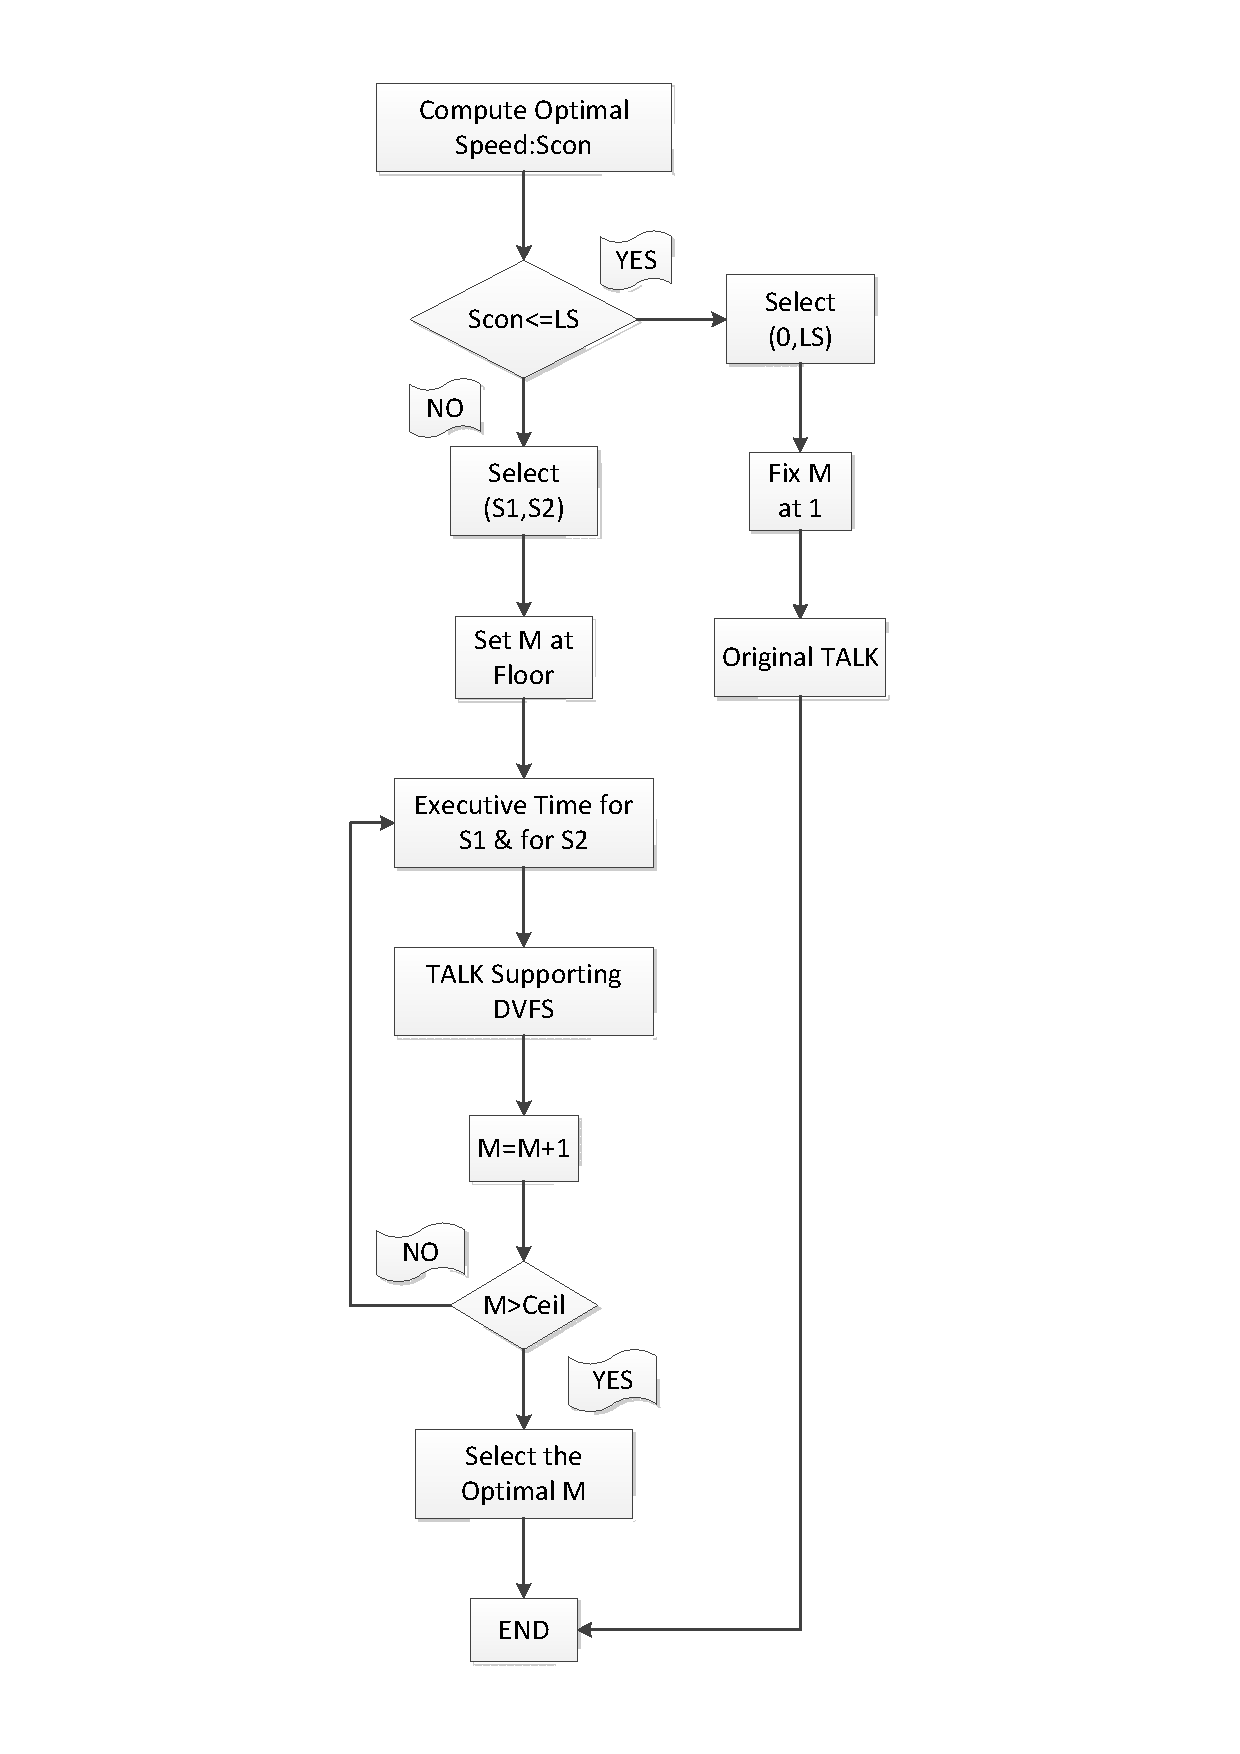
\includegraphics[width=0.8\textwidth,height=0.8\textheight]{Visio-VS-TALK}
  \caption{VP-TALK算法流程}
  \label{fig:vp-talk}
\end{figure}
与MO相似,VP-TALK首先需要假设电压可以连续调节、以获得理论上的最优工作速度$S_{con}$。在$S_{con}\leq LS$(芯片最低工作速度)时, VP-TALK等同于原始的TALK算法。在$S_{con}>{LS}$时,该算法选用两档邻接的速度$S_1$和$S_2$,使得$S_1\leq S_{con}<S_2$。 不同于MO的等分$M$段时间段,VP-TALK采用更灵活的、电压可调的温敏TALK来对每一小段的工作状态进行调度。 由于$m$的数量由切换工作状态的代价和任务的实时性所限制, 其上下限分别记为$Ceil$和$Floor$\onlinecite{LkEngMinRTSysMaxTemConst}。 VP-TALK的应用前提是假设我们已经通过某种预测的方法预测出了任务负载量,从而,在任务到达前调度就已经开始, 所以认为是实时性的。

\section{DPTM原型系统}
\label{DPTM-system}
\subsection{启发性示例}
在之前的分析中,我们已经指出,较轻工作负载时的MO必然要退化至PB的方法. 这是因为当工作所需电压低于可选的最小电压值时,MO中阶梯型工作电压策略无法通过逼近最优工作电压的方式节省动态功耗。 为了探究工作量与最优调度算法之间的关系,我们设定任务长度为10秒, 并考虑比文献\onlinecite{LkEngMinRTSysMaxTemConst}更强的温度对漏电流影响, 我们在工作负载率全区间(5\%-95\%)范围内,对TALK、PB与MO这3种已有调度源算法的调度效果进行了考察。 图\ref{fig:exp-power-cmp}给出了能耗的数据,图\ref{fig:exp-temp-cmp}给出了温度数据。
\begin{figure}%[H] % use float package if you want it here
  \centering
  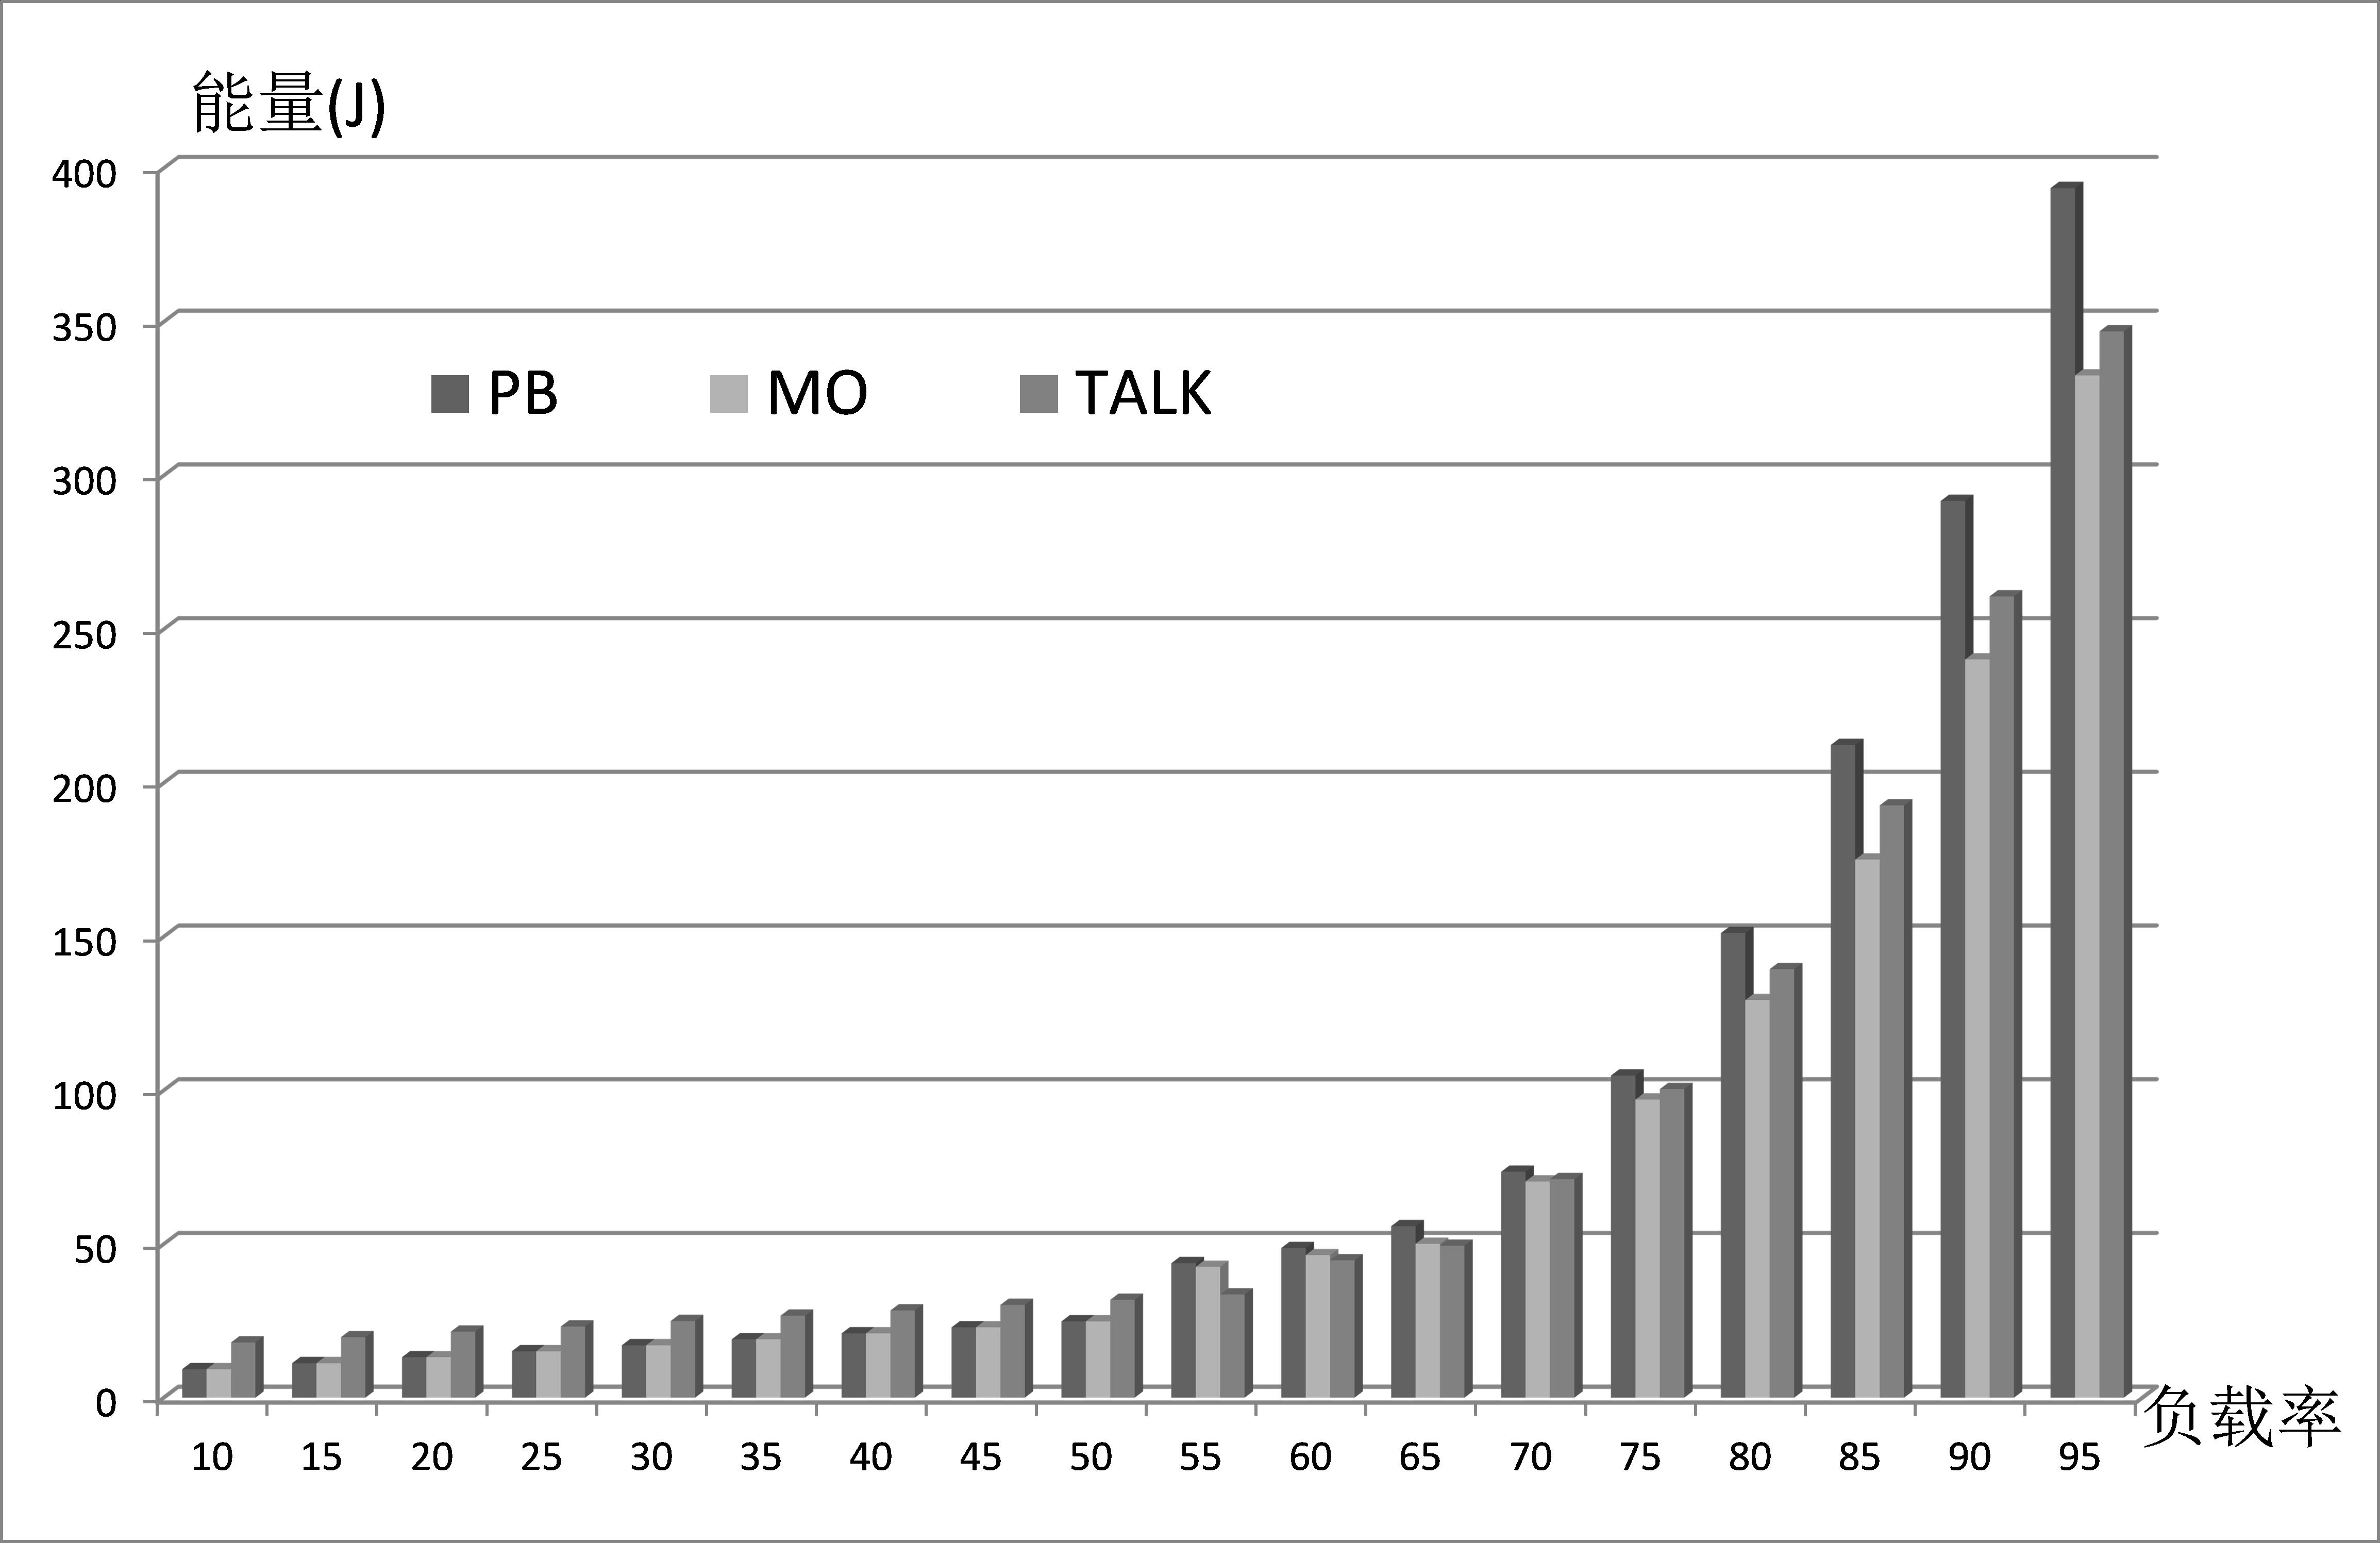
\includegraphics[width=1.0\textwidth]{power_cmp}
  \caption{不同负载率下已有调度算法的能耗比较}
  \label{fig:exp-power-cmp}
\end{figure}
\begin{figure}%[H] % use float package if you want it here
  \centering
  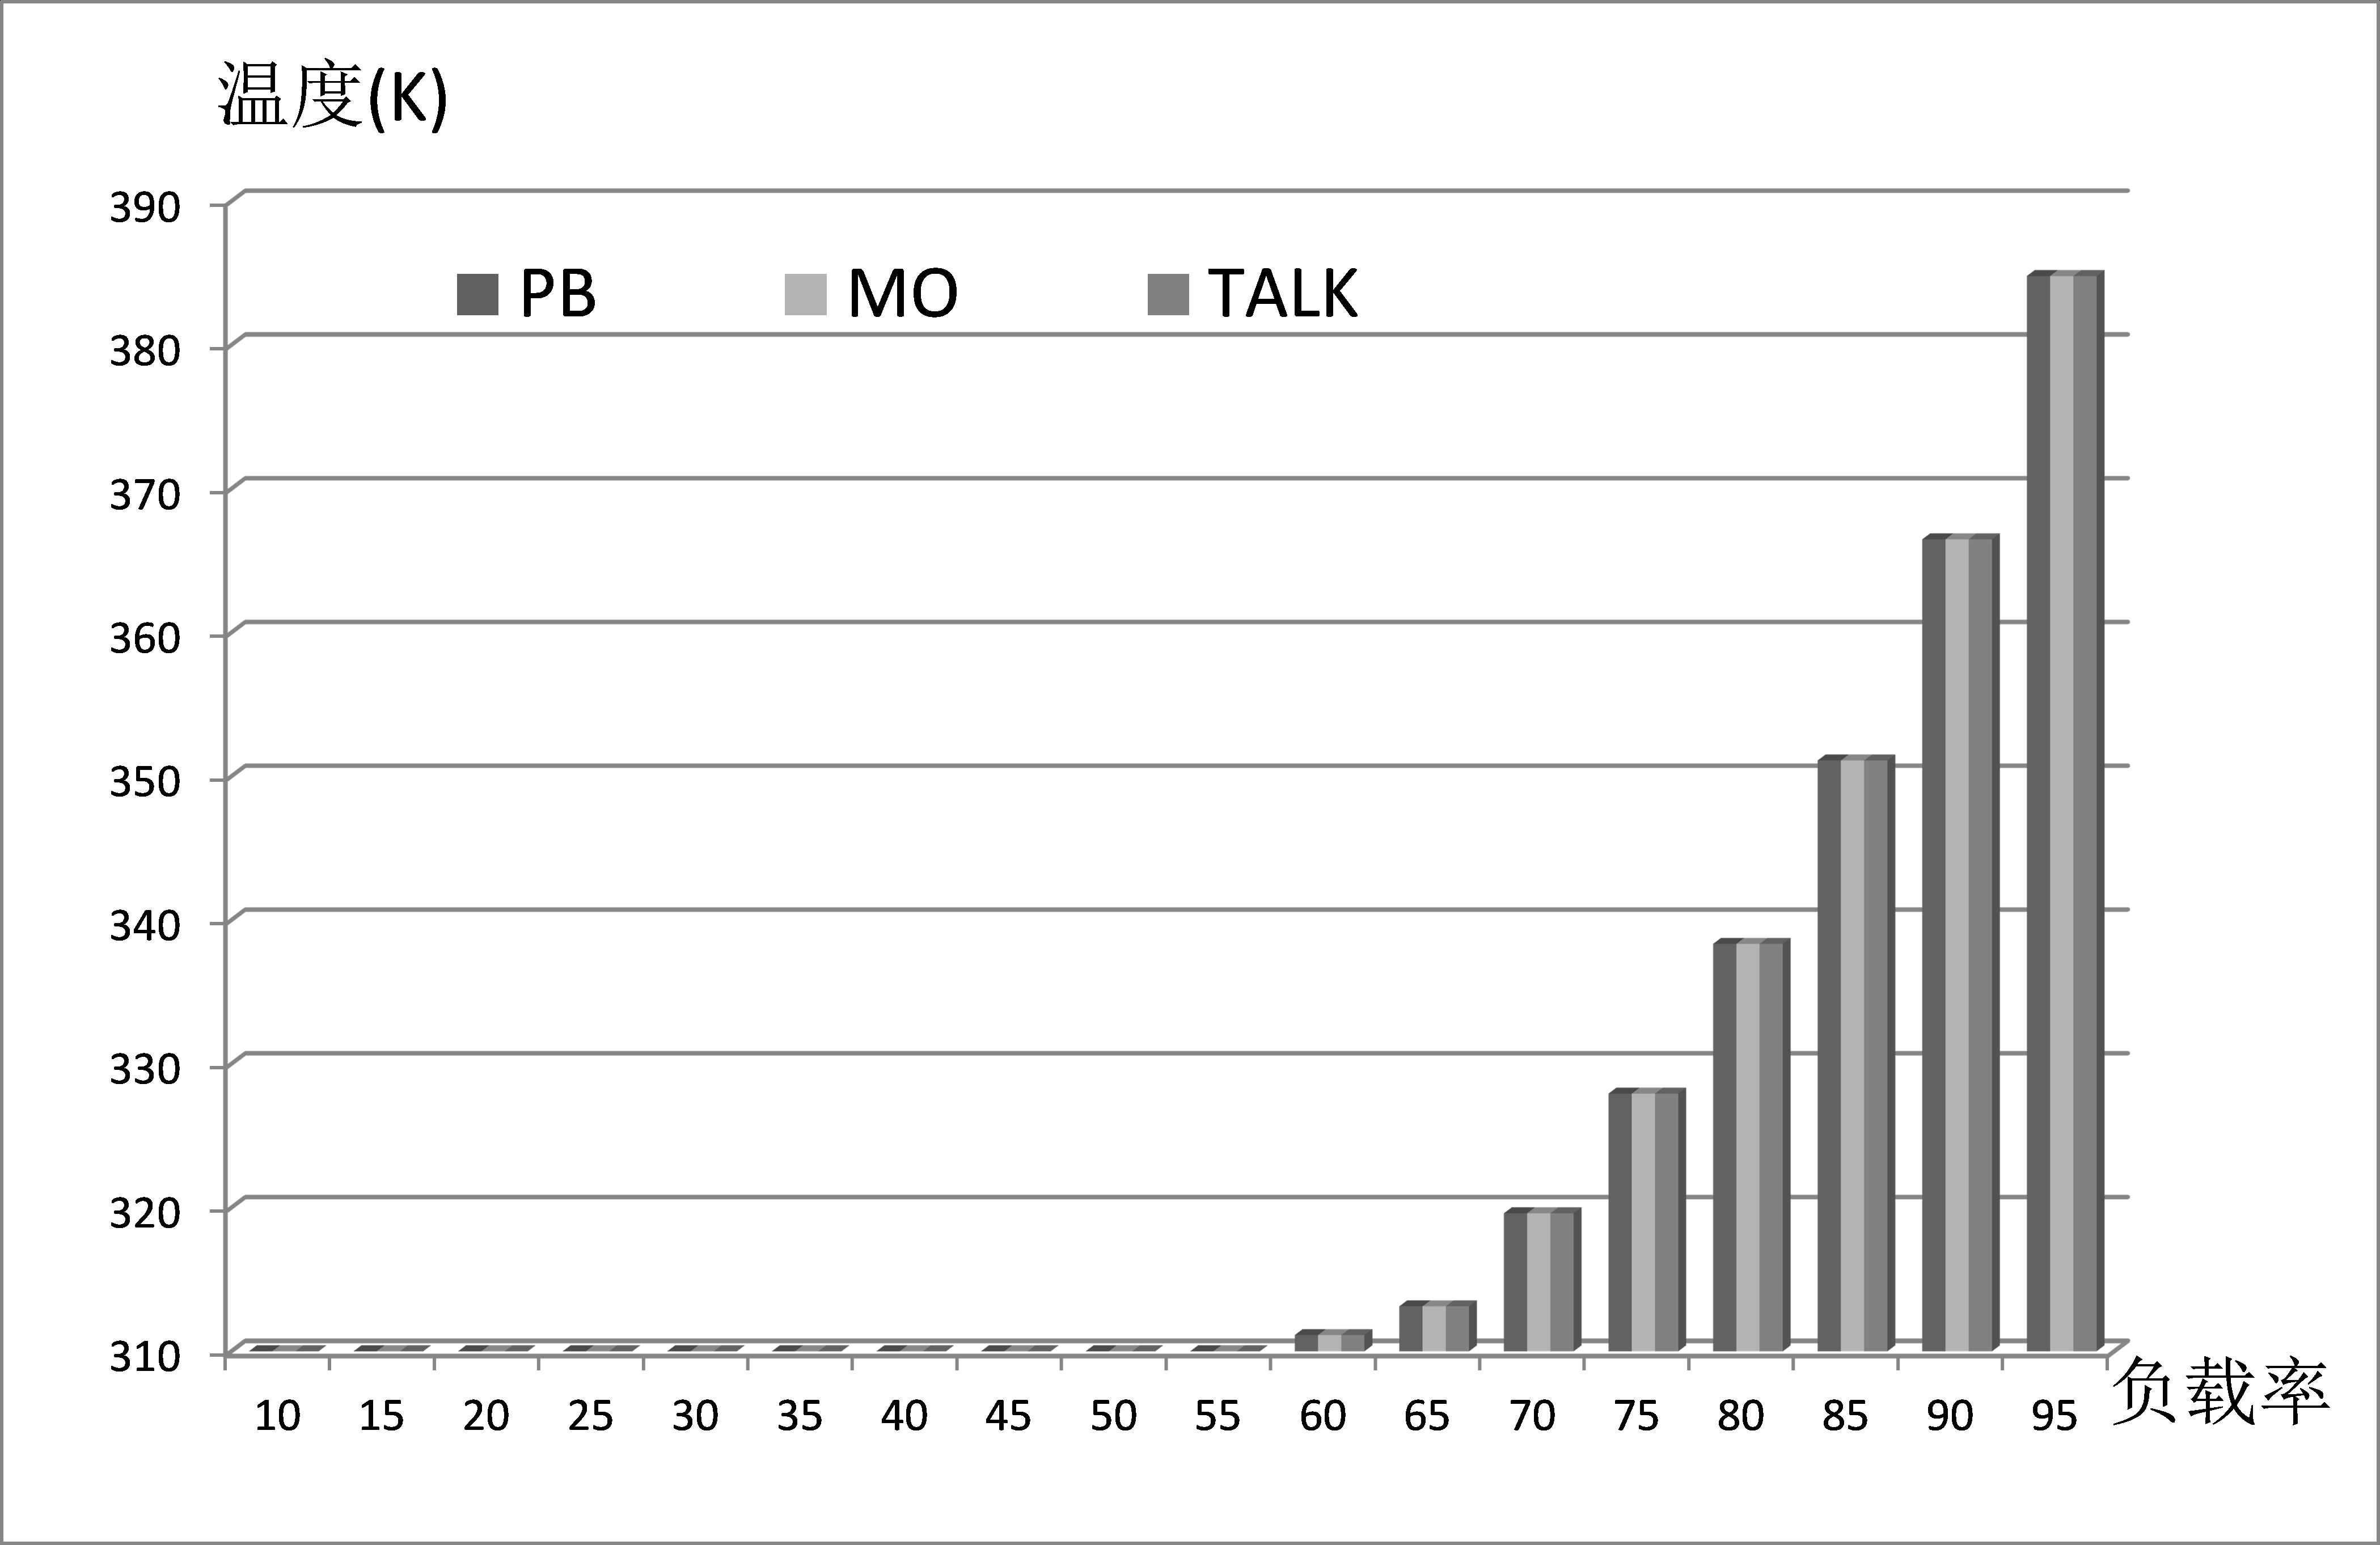
\includegraphics[width=1.0\textwidth]{temp_cmp}
  \caption{不同负载率下已有调度算法的温度比较}
  \label{fig:exp-temp-cmp}
\end{figure}
我们可以得出如下结论:
(1)	当工作负载率($W/D$)低于50\%(近似值)时,三种源算法的峰值温度低于310K(37 C),峰值温度对系统的性能与可靠性没有影响;在系统能耗方面,PB算法(也即MO算法)的调度效果要胜过TALK算法, 因此,PB算法具有最佳的调度效果。
(2)	当工作负载率($W/D$)处于50\%-70\%区段(近似值)时,三种源算法的峰值温度低于320K(47 C),峰值温度对系统的性能与可靠性也没有影响;在系统能耗方面,TALK算法的调度效果要胜过PB和MO算法, 因此,TALK算法具有最佳的调度效果。
(3)	当工作负载率($W/D$)大于70\%(近似值)时,三种源算法的峰值温度高于320K(47 C),最高可超过380K(107 C),峰值温度对系统的性能与可靠性具有明显影响,其中MO算法具有最低的峰值温度;在系统能耗方面, MO算法的调度效果要明显胜过其它两种源算法,MO算法具有最佳的调度效果。
由此可见,最优的DPTM调度算法与工作负载率有直接关系。我们将以此关系作为理论基础,用于DPTM调度原型系统的构建, 即根据对实时系统工作负荷的精确预测结果,来选择效果最佳的调度算法,并对DPTM调度效果进行评价。

\subsection{基于机器学习的DPTM原型系统}
根据调度算法性能与工作负载大小相关的观察,我们提出了基于工作负载预测结果来选择DPTM调度算法的调度策略, 并以此构建了本文的DPTM原型系统,整个系统由工作负载预测、调度策略选择和调度策略评价三大模块组成, 其具体的架构及其工作原理如图4所示。
在该系统工作中,其三大模块主要完成如下功能。 (1)工作负载预测模块:我们根据负载变化周期的长短,提出了一种组合式的负载预测方法, 采用多种不同拟合方法来分别对任务的不同物理意义成分进行精确预测,以获得对复杂任务的精确预测; (2)调度策略选择模块:我们综合考虑实时完成任务、温度上限、能耗最小化、 漏电流与温度相关以及芯片模式切换代价等多种因素, 选用不同的任务调度策略; (3)调度策略评价模块:对每种策略的系统能耗与峰值温度进行评价,并将其作为DPTM系统的反馈量,供调度策略选择模块参考。
调度策略选择的学习主要通过后期性能评价的评价值完成。假设存在$N$类DPTM,编号为$1,2,……,N$。 它们在某一时刻$t$的得分或者权重为,$w_t=(w_{1t},w_{2t},...,w_{Nt})$对其中任一个权重分量$w_{kt}$可以 采用式\ref{equ:chap2:cal-weight}进行计算
\begin{equation}
\label{equ:chap2:cal-weight}
w_{kt} = 1- \sum\limits_{j=t_0}^{t-1} \frac{E_{k,j}\lambda_j}{\sum\limits_{i=1}^N E_{i,j}}
\end{equation}
式\ref{equ:chap2:cal-weight}中$E_{i,j}$代表芯片使用第$i$类DPTM在时刻$j$的负载情况下消耗的能量, $\lambda_{j}$为一可调整的参数, 代表时刻$j$的能耗情况对决策的影响程度,$t_0$是可以变动的初始值, 它的取值意味着选取从何时开始的能耗情况作为以后决策的参考。在预测出工作负荷值后, 则开始使用\ref{equ:chap2:decide}进行决策:
\begin{equation}
\label{equ:chap2:decide}
DPTM_t = \arg(\max\limits_{1\le k \le N}(w_{k,t}))
\end{equation}
式\ref{equ:chap2:decide}中$DPTM_t$为$t$时刻选择出的动态功耗温度调度策略。考虑到温度上的限制, 我们需要考察所选的调度源算法是否会超过温度上限。 如果能耗的节约是在很高的峰值温度的代价下换取的,我们将放弃该源算法,而选择次优的但是有较低峰值温度的调度源算法。
与三种已有源算法和本文提出的VP-TALK算法相比,本文DPTM系统的主要扩展改进点在于: 具有高精度的任务预测模块,为根据负载量而进行的策略选择提供前提基础; 通过基于调度效果评价的机器学习,自适应地根据负载量的轻重选择调度策略。

\subsection{基于单一调度策略的DPTM原型系统}
值得一提的是,如果我们选定某一种调度策略,省略机器学习模块,就构成了基于单一调度策略的DPTM原型系统。 在该DPTM原型系统中,输入量为任务负载的历史值,通过这些历史值,利用第六节所述的任务负载预测模型, 可以得到对于下一时刻任务量的预测值。 进而,可以确定完成预测任务值所需要的芯片电压或者频率,并利用上文所述的某一种算法进行调度。
不论是基于及其学习的DPTM系统,还是基于单一调度策略的DPTM系统,都要求提前预知任务负载的大小。 因此,本文采用所提出的组合模型预测方法。该方法将复杂任务按频谱长短分类为随机/周期/趋势等三种成分, 然后采用灰色模型/傅里叶模型/径向基函数(RBF)神经网络模型对这三种成分进行组合分析, 可以得到平均相对误差低于3\%、归一化方差小于0.5的任务负载预测效果\onlinecite{DPTMbyYJQ}。 

%%% Local Variables:
%%% mode: latex
%%% TeX-master: t
%%% End:

% !Mode:: "TeX:UTF-8"

\chapter{DPTM原型系统模拟实验}
\label{cha:DPTMexperiments}

\section{模拟实验环境}
为了验证本文所提出的预测任务负载模型、VP-TALK调度算法以及DPTM原型系统,我们进行了三组模拟实验。实验运行平台为配有Intel Core 2 Q9550 CPU、4GB RAM的Windows7 64位操作系统,预测模型以及各DPTM算法在MATLAB\onlinecite{MATLAB}软件中模拟实现。

\section{VP-TALK算法的DPTM效果验证}
本文通过与现有的TALK、PB、MO算法进行对比,来验证本文提出的VP-TALK算法的优越性。 实验中选取$p_r$、$c_r$取值分别为0.001$s$/$V$和0.01$J$/$V^2$,温度最高上限设为390K,任务周期固定为10$s$。 支持DVFS芯片的电压值从0.6$V$到1.4$V$可调,步长0.1$V$。根据电压可以得到归一化的速度序列为{0.574, 0.6611, 0.7324, 0.7926, 0.8446, 0.8901, 0.930, 0.9670, 1}。 任务负载率为5\%至95\%,变化步长为5\%。 对于4种对比算法,我们分别将能耗情况(单位为焦耳$J$)和峰值温度情况(单位为绝对温度$K$)绘制于 图\ref{fig:vp-talk-power-cmp}和图\ref{fig:vp-talk-temp-cmp}。
\begin{figure}[H]
  \centering
  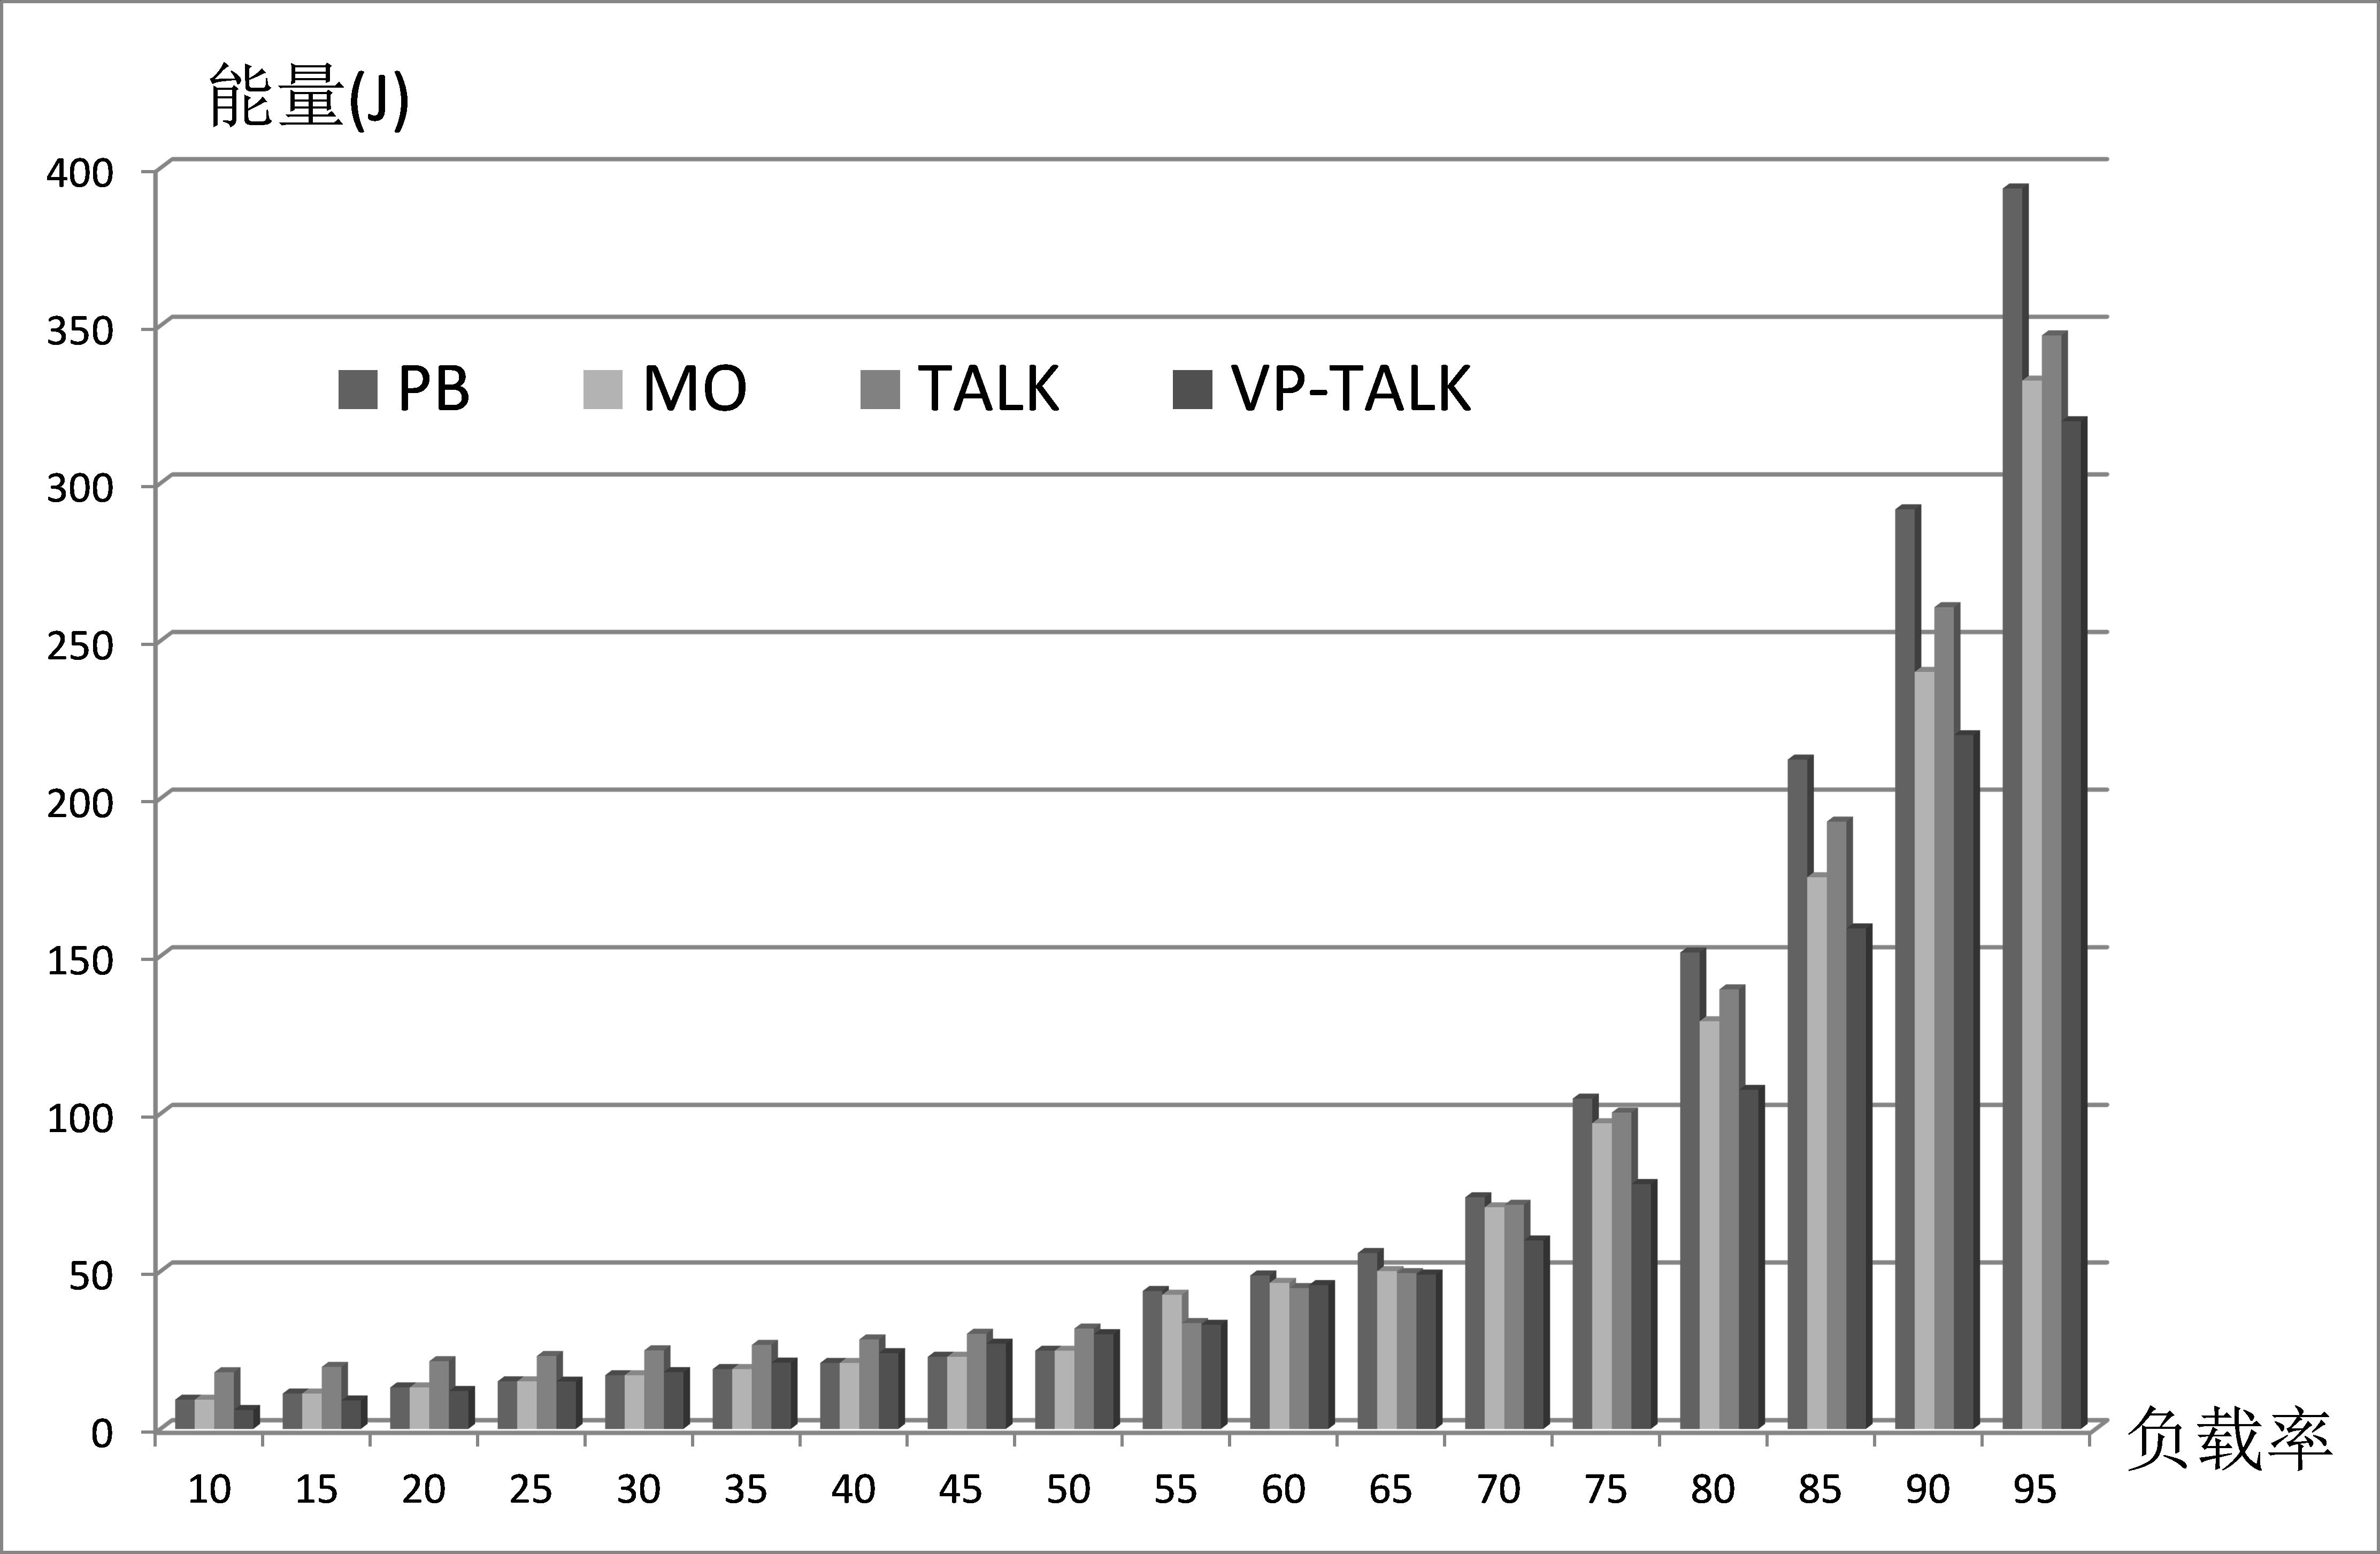
\includegraphics[width=1.0\textwidth,height=0.5\textheight]{VP-TALK-POWER-CMP}
  \caption{能耗比较}
  \label{fig:vp-talk-power-cmp}
\end{figure}
\begin{figure}[H]
  \centering
  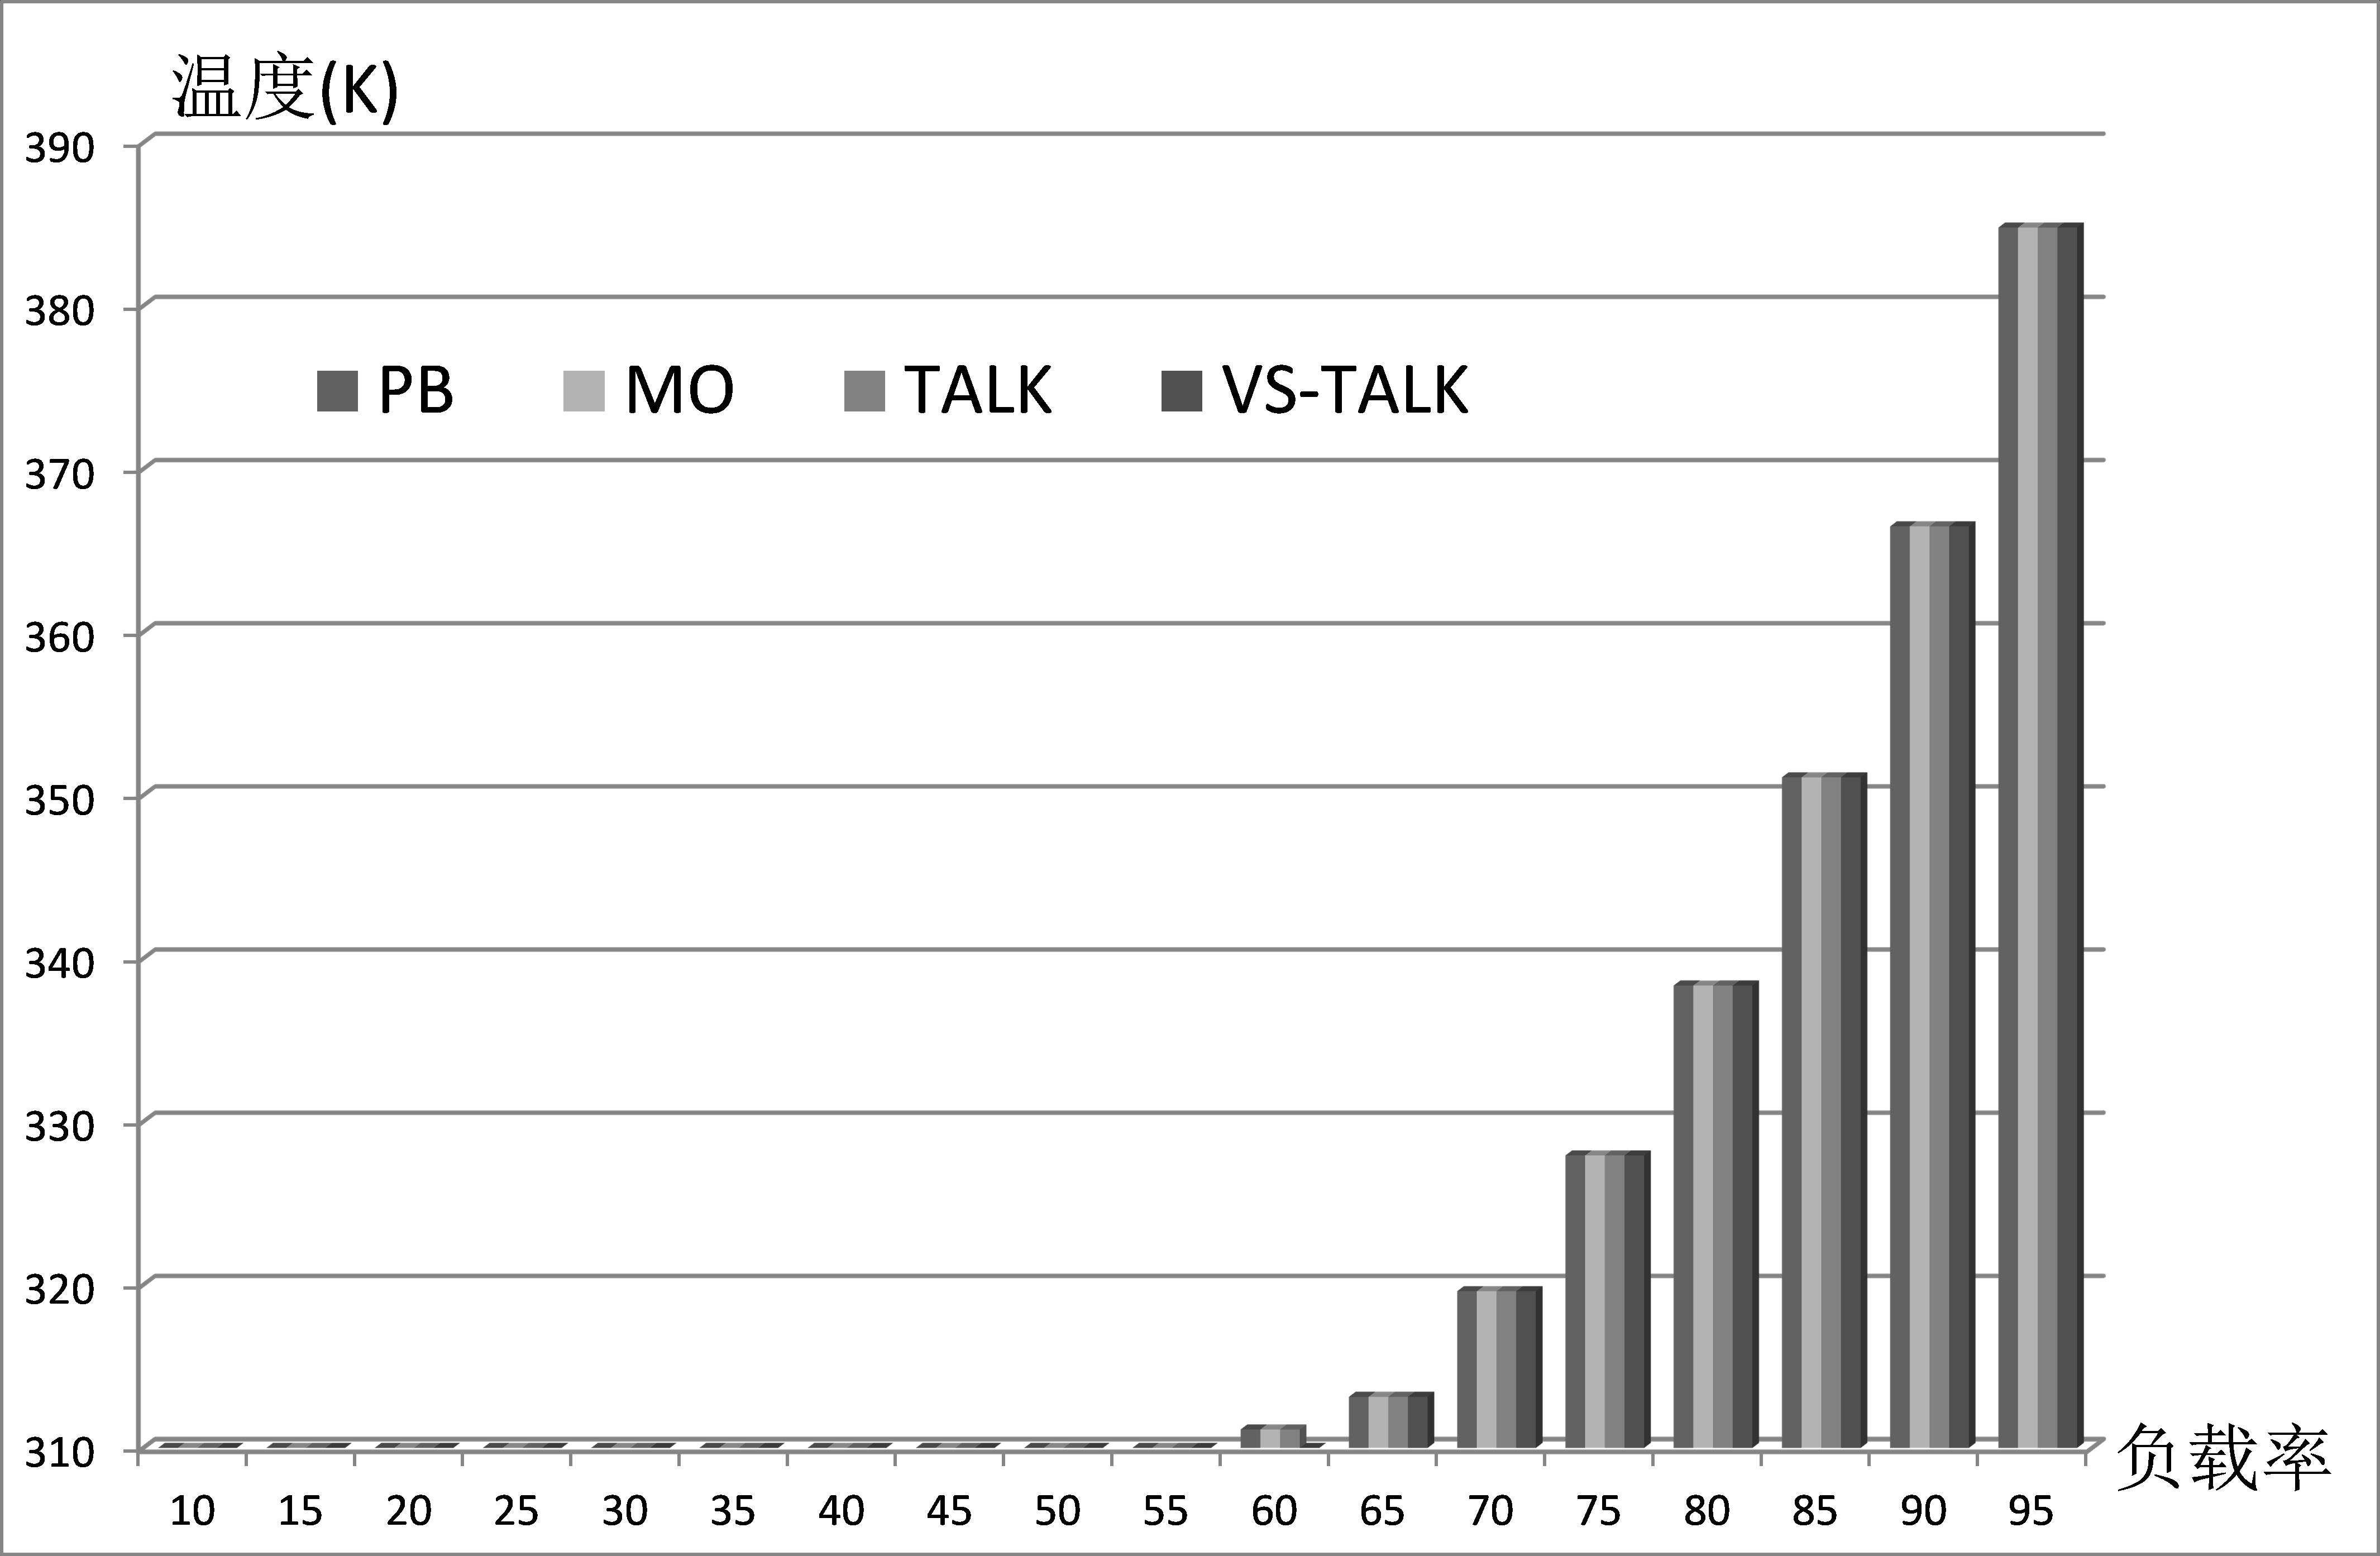
\includegraphics[width=1.0\textwidth,height=0.5\textheight]{VP-TALK-TEMP-CMP}
  \caption{峰值温度比较}
  \label{fig:vp-talk-temp-cmp}
\end{figure}
从图\ref{fig:vp-talk-power-cmp}可以看出,对于能耗:当负载率小于55\%时,VP-TALK优于TALK、PB与MO等价。 这是因为,在负载率不高于芯片最低运行速度(0.574)时,VP-TALK相当于使用DVS技术的TALK,PB相当于使用单一速度的MO。 此时,TALK与PB的调度效果相差无几。在负载率为25\%到50\%时,PB略优于VP-TALK算法。 原因是VP-TALK在电压和时间切换上付出了更大的代价。 然而,随着负载率的增加,当负载率大于55\%时,VP-TALK的调度效果全面优于其他三种算法, 比PB、MO以及TALK的平均能耗分别节省大约20.54\%、11.04\%、11.42\%。表\ref{tab:chap3:vp-talk-cmp}列出了当负载率大于55\%时,能耗节省数据的统计信息, 具体说明了VP-TALK的在能耗节约方面的优势。
从图\ref{fig:vp-talk-temp-cmp}中可以看出,当工作负载率小于50\%时,各种算法所达到的峰值温度都不超过310$K$, 四种调度算法在峰值温度方面的差距基本小于1$K$,并在最大负载率时近似共同终结于384$K$。

\begin{table}
\centering
\caption{VP-TALK相对于已有算法的节能情况}
\begin{tabular}{c c c c c}
\hline\hline
算法 & PB & MO & TALK & Avg \\ [0.5ex]
\hline
平均(\%) & 20.54 & 11.04 & 11.42 & 14.33 \\
最大(\%) & 28.83 & 22.34 & 21.27 & 24.68 \\
\hline
\end{tabular}
\label{tab:chap3:vp-talk-cmp}
\end{table}

\section{基于机器学习的DPTM原型系统的验证}
为了评价本文基于机器学习的DPTM原型系统功耗与温度的调度效果,我们做了两组实验。
首先,基于\onlinecite{DPTMbyYJQ}中所得到的每个时刻工作负载预测值,我们分别采用四种对比源算法, 即TALK\onlinecite{TemLkMinTechRTSys}、PB\onlinecite{EngRTTskSchTemDepLk}、 MO\onlinecite{LkEngMinRTSysMaxTemConst},VP-TALK, 算出每个时刻每种算法的能耗值与峰值温度; 然后将四种对比源算法每个时刻的能耗值与峰值温度进行平均,得到四种对比源算法每个时刻的平均调度效果; 最后使用图\ref{fig:dptm-source-alg-power-cmp}与图\ref{fig:dptm-source-alg-temp-cmp}分别 比较了本文原型系统与四种对比源算法平均调度效果的能耗(单位$J$)和峰值温度(单位$\celsius$)。
\begin{figure}[H]
  \centering
  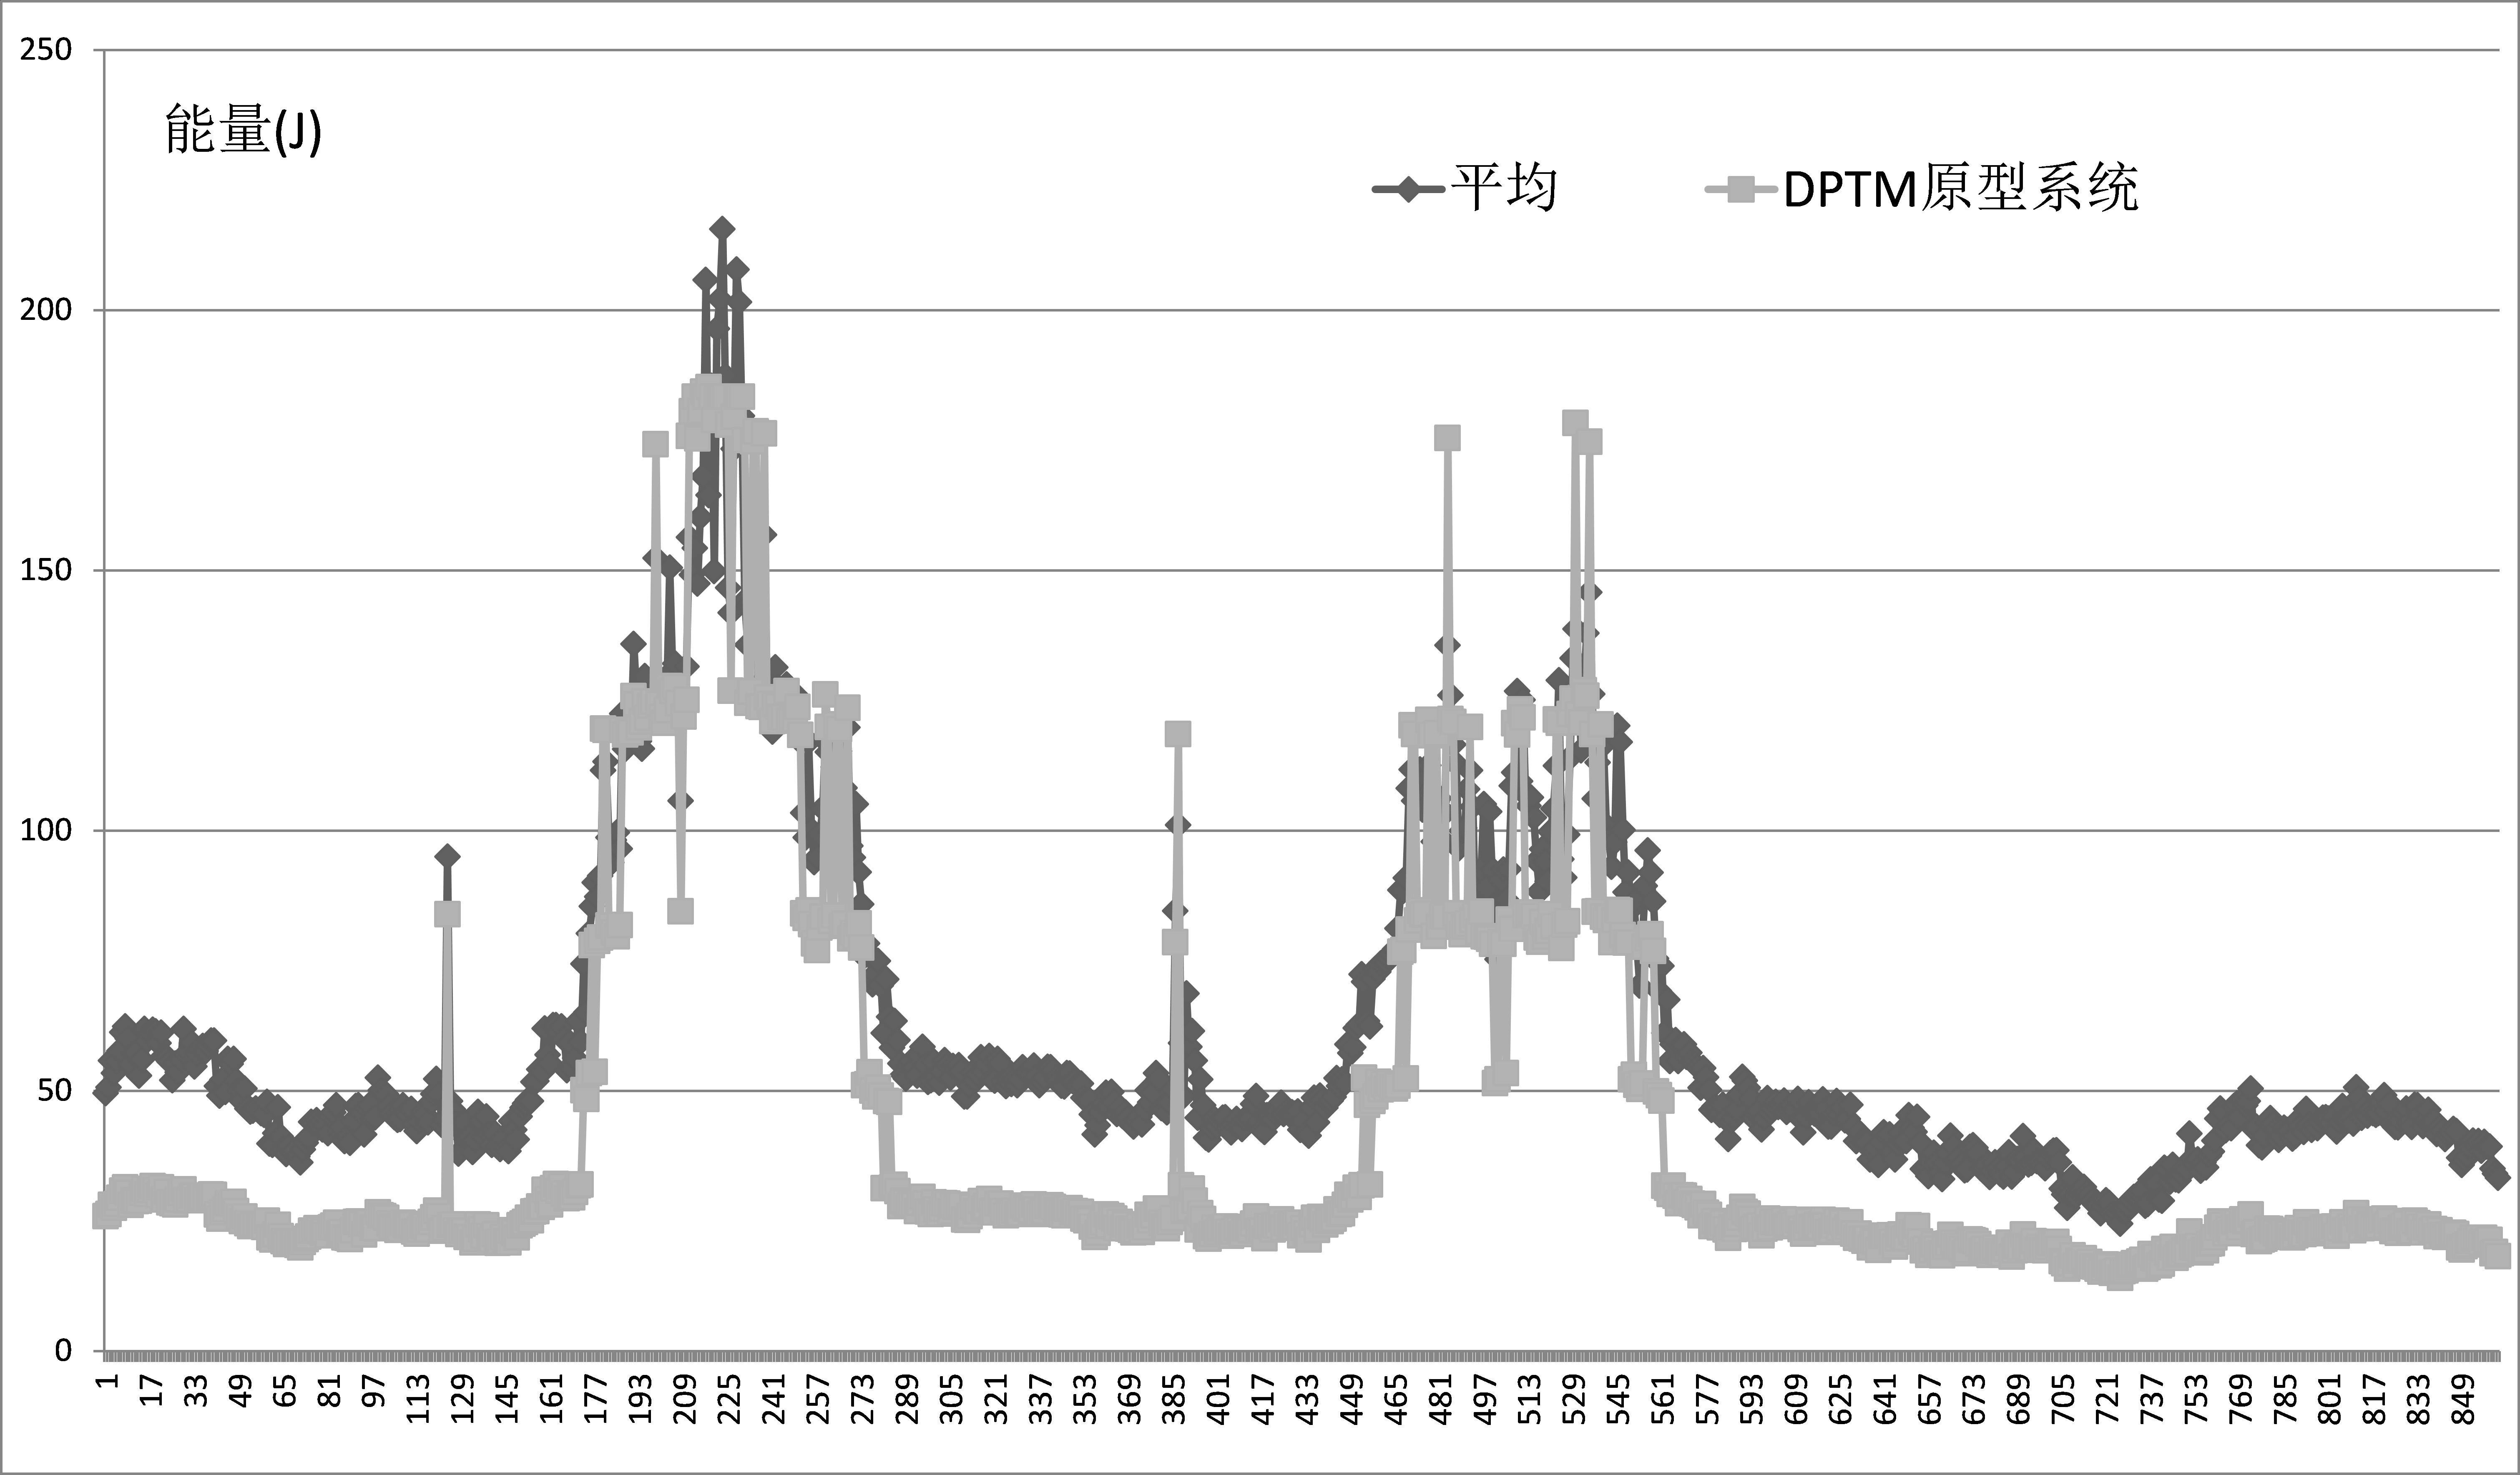
\includegraphics[width=1.0\textwidth,height=0.4\textheight]{DPTM-SOURCE-ALG-POWER-CMP}
  \caption{DPTM原型系统VS源算法均值(能耗)}
  \label{fig:dptm-source-alg-power-cmp}
\end{figure}
\begin{figure}[H]
  \centering
  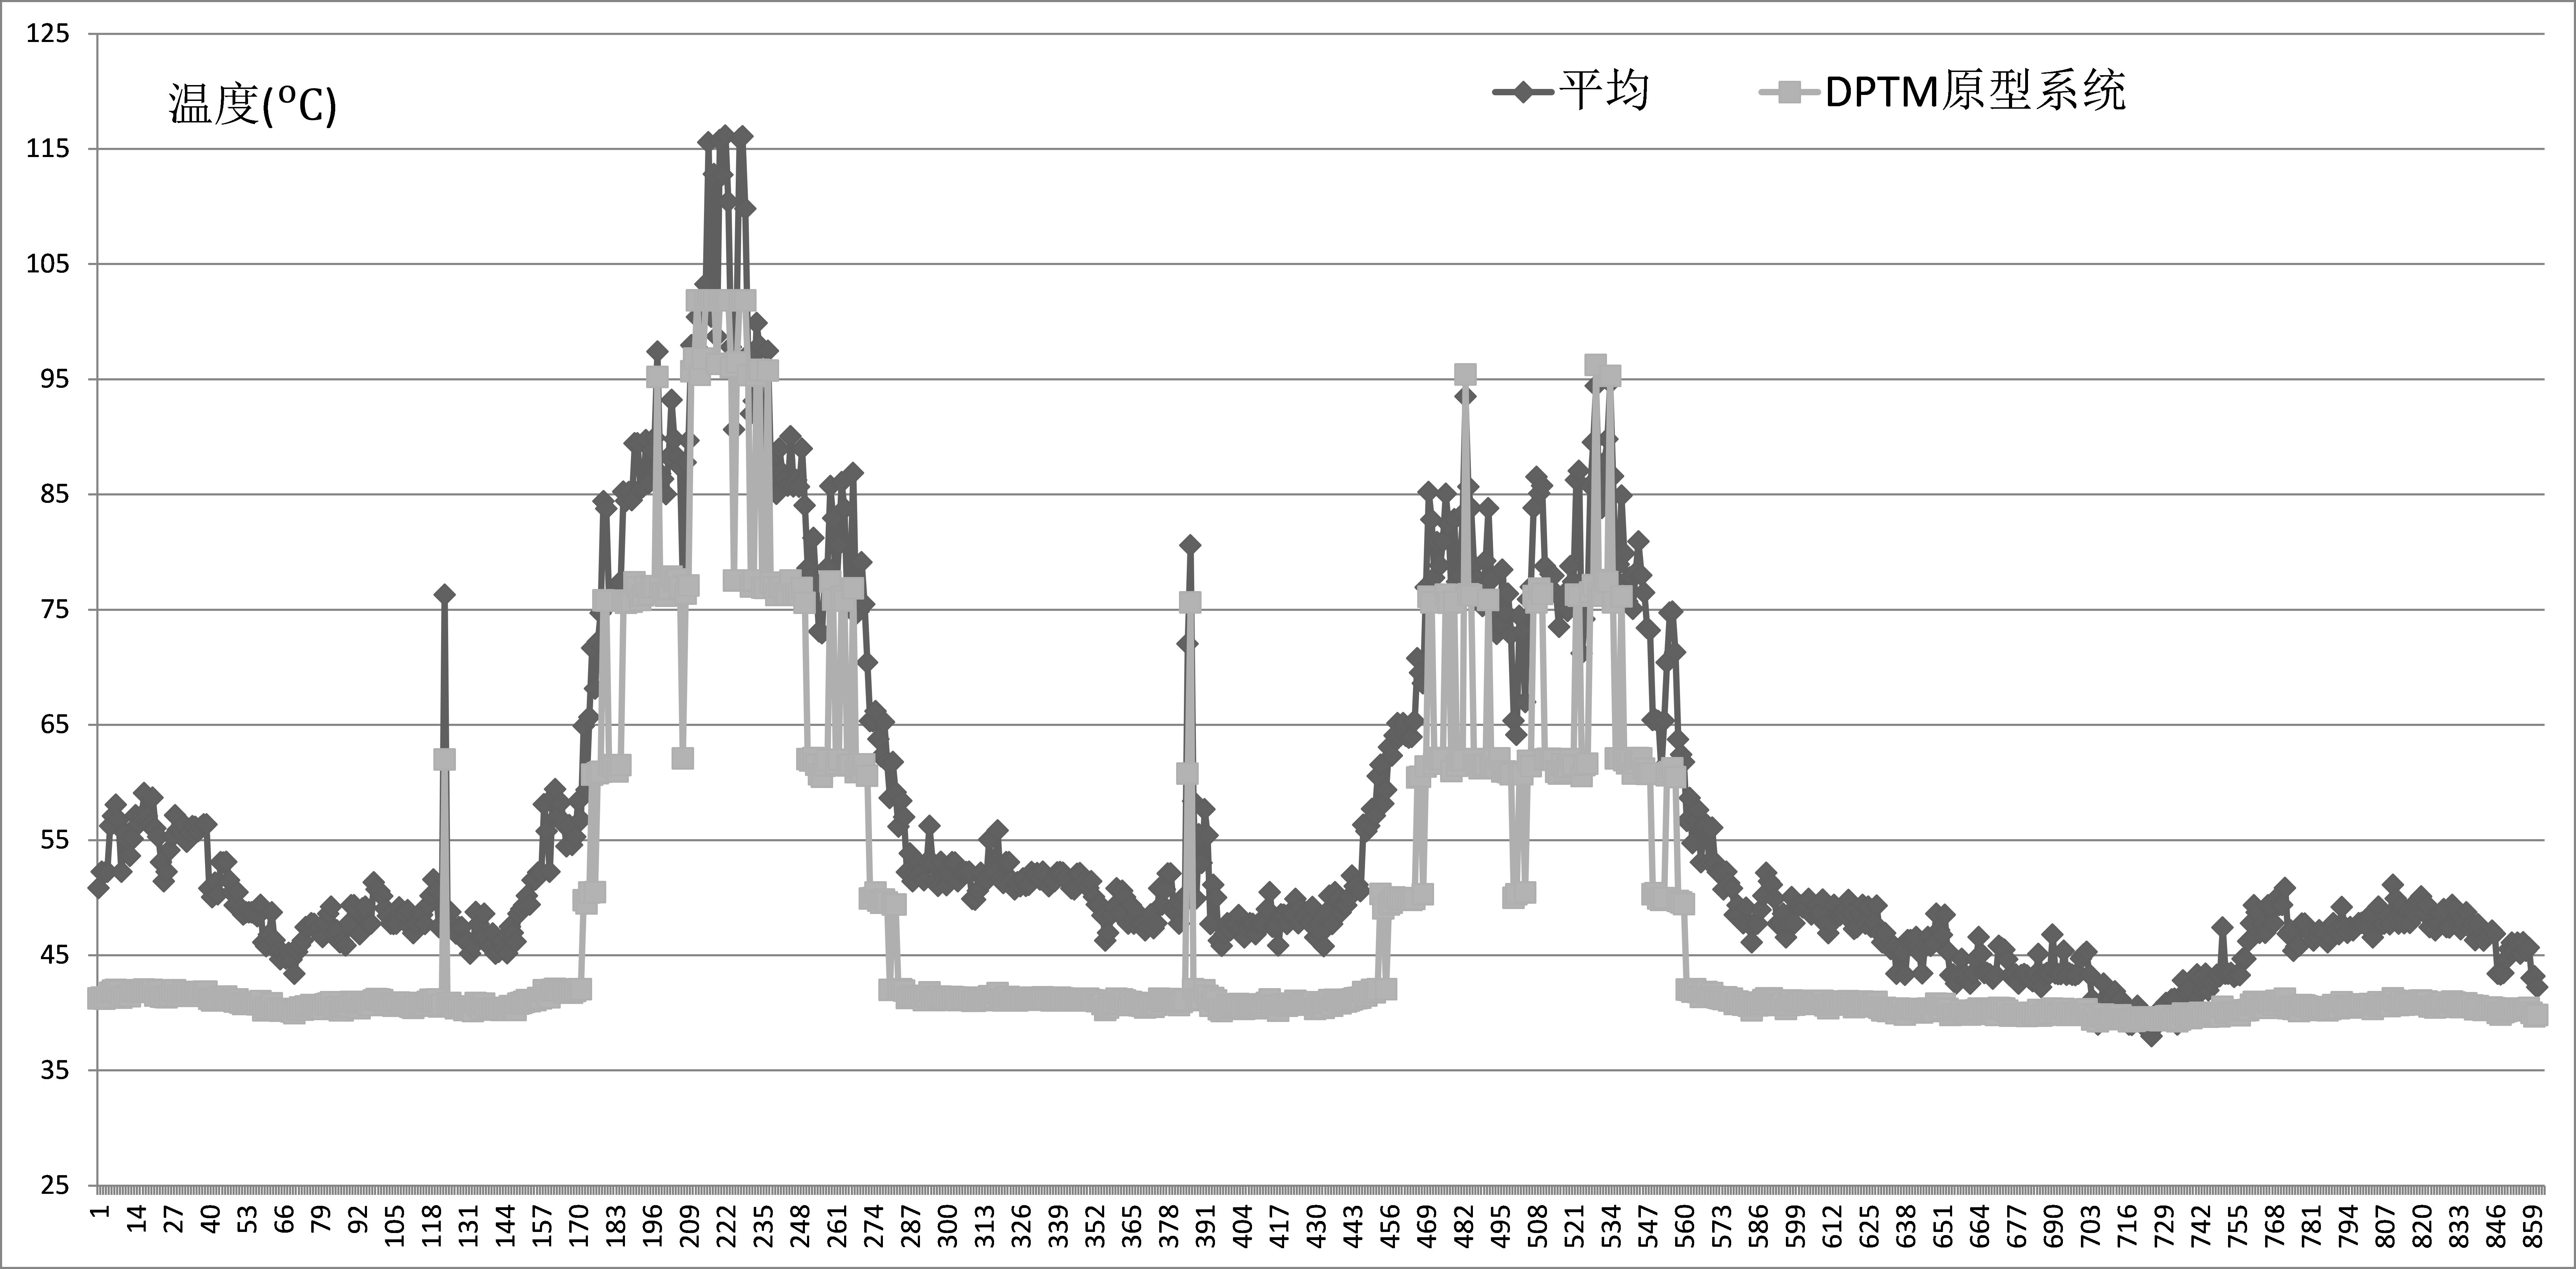
\includegraphics[width=1.0\textwidth,height=0.4\textheight]{DPTM-SOURCE-ALG-TEMP-CMP}
  \caption{DPTM原型系统VS源算法均值(峰值温度)}
  \label{fig:dptm-source-alg-temp-cmp}
\end{figure}
\begin{figure}[H]
  \centering
  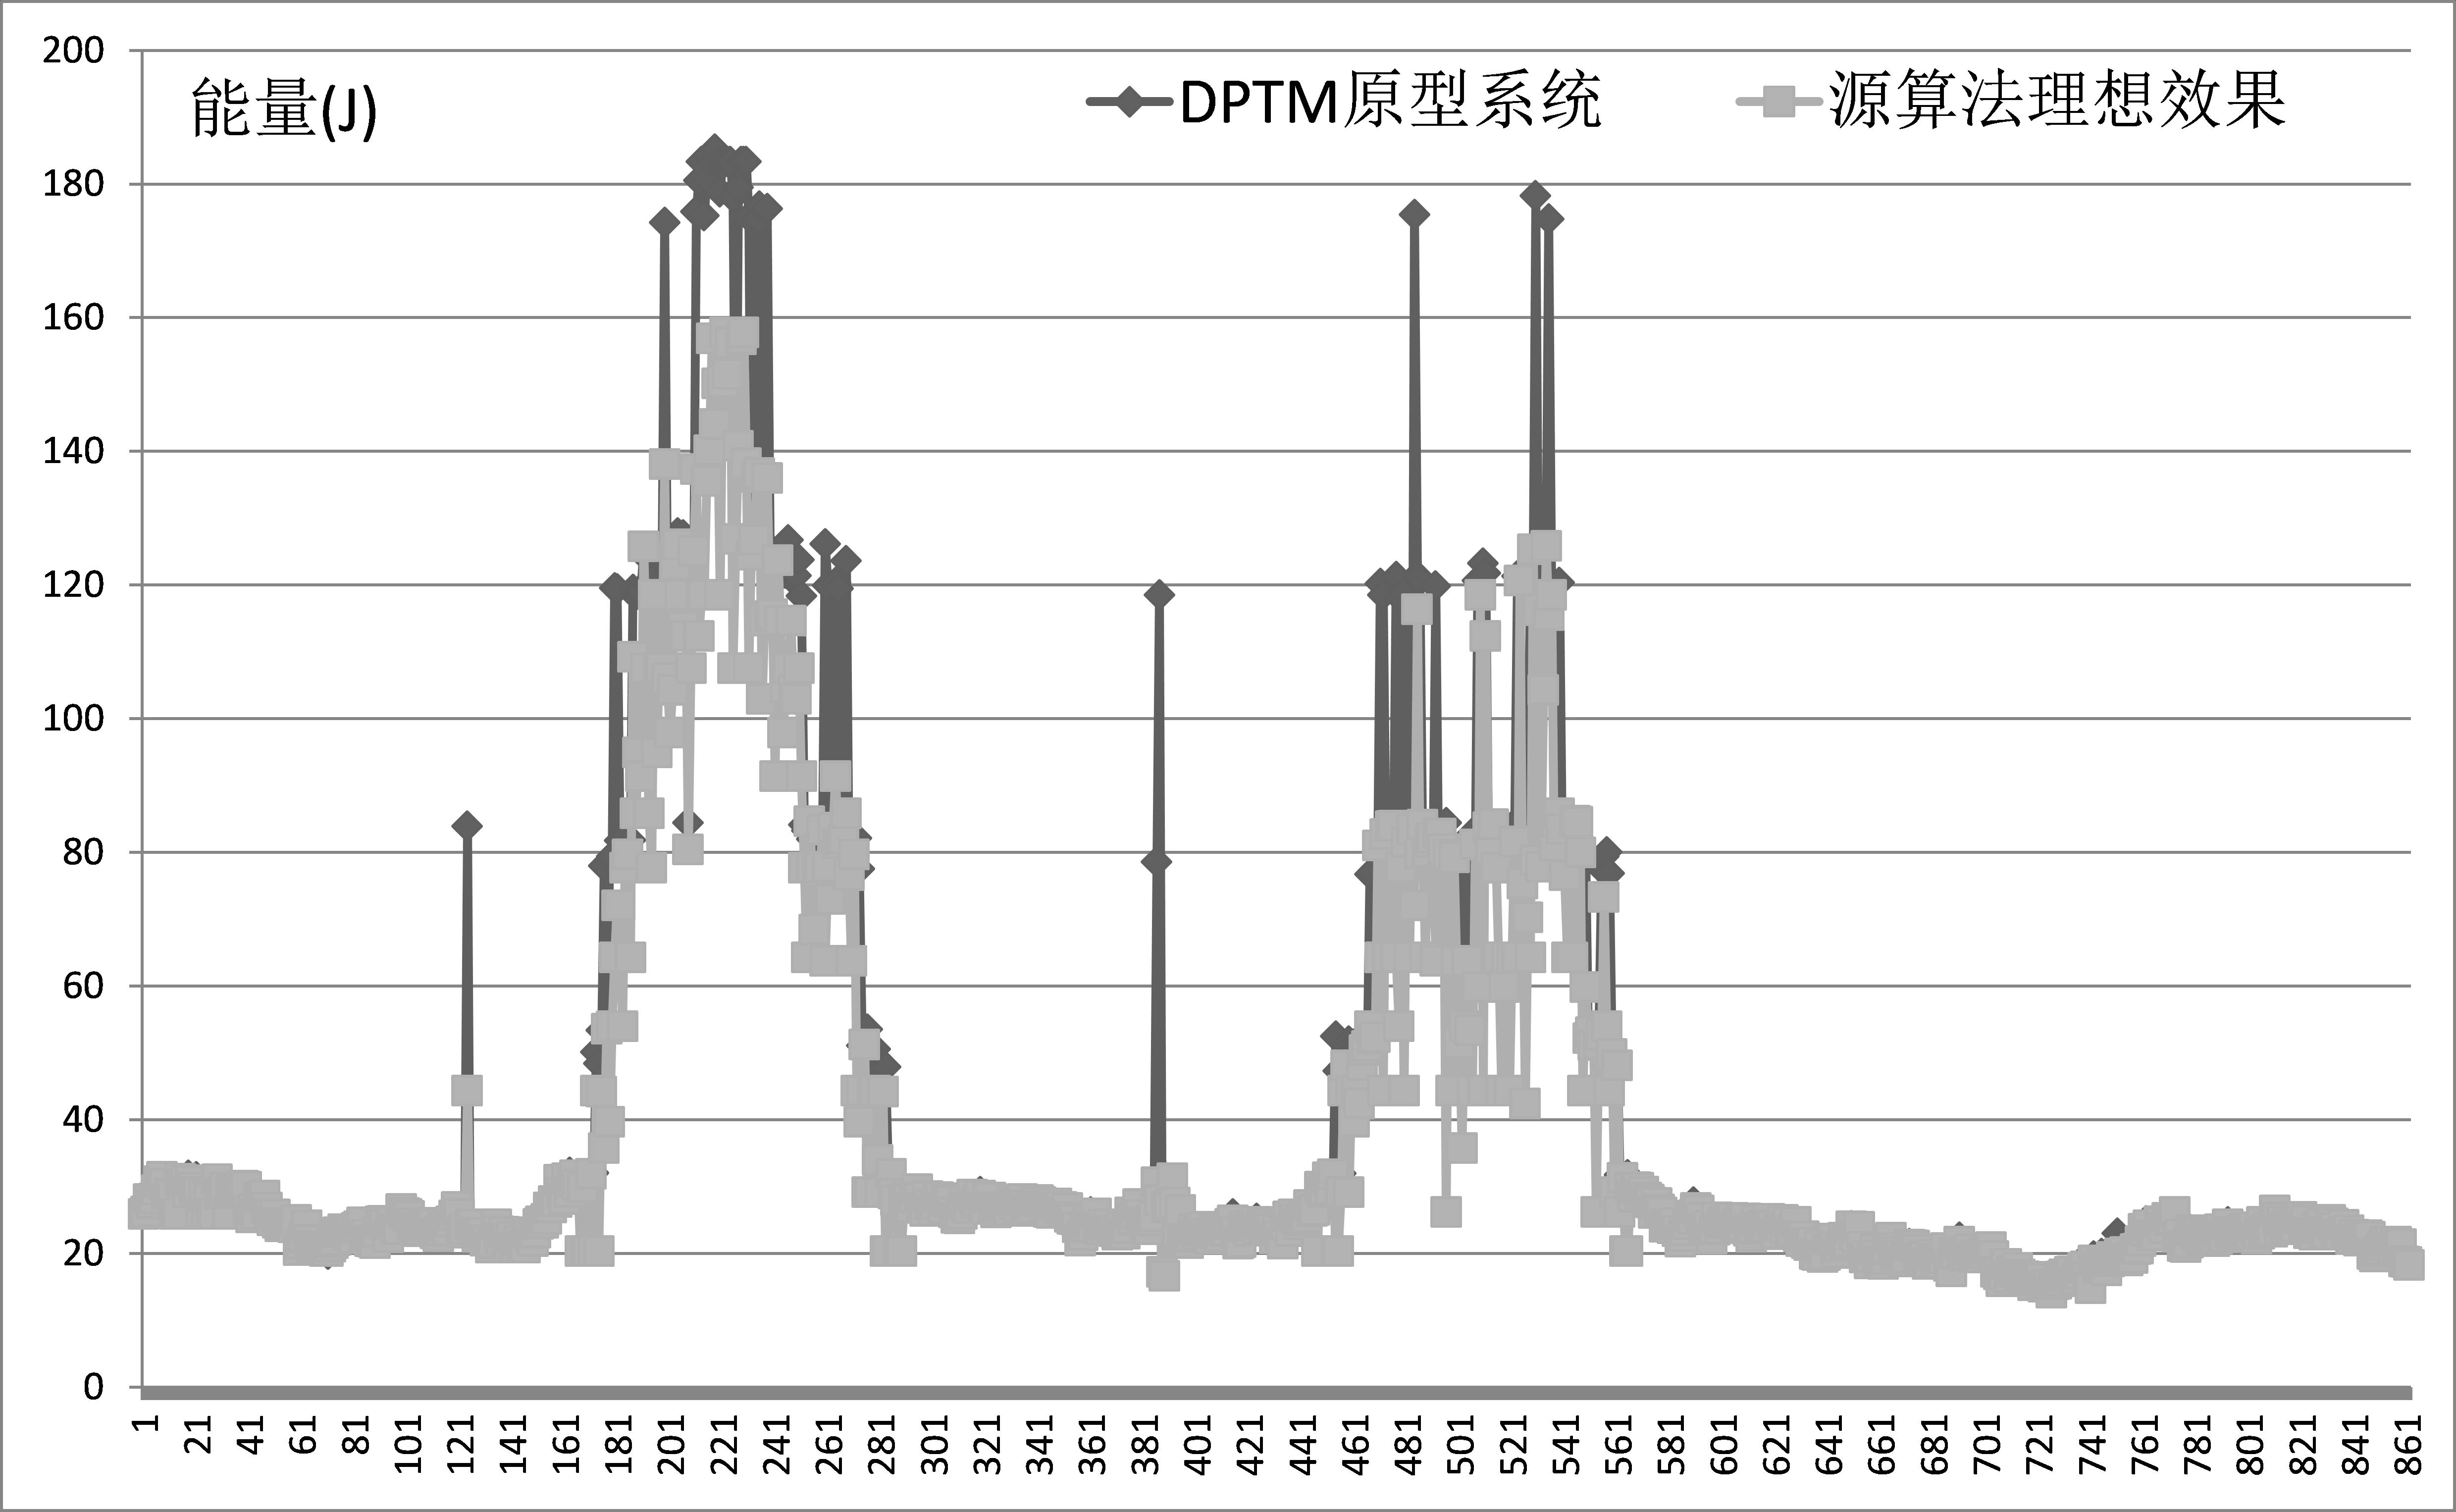
\includegraphics[width=1.0\textwidth,height=0.4\textheight]{DPTM-IDEAL-POWER-CMP}
  \caption{DPTM原型系统VS理想效果(能耗)}
  \label{fig:dptm-ideal-power-cmp}
\end{figure}
\begin{figure}[H]
  \centering
  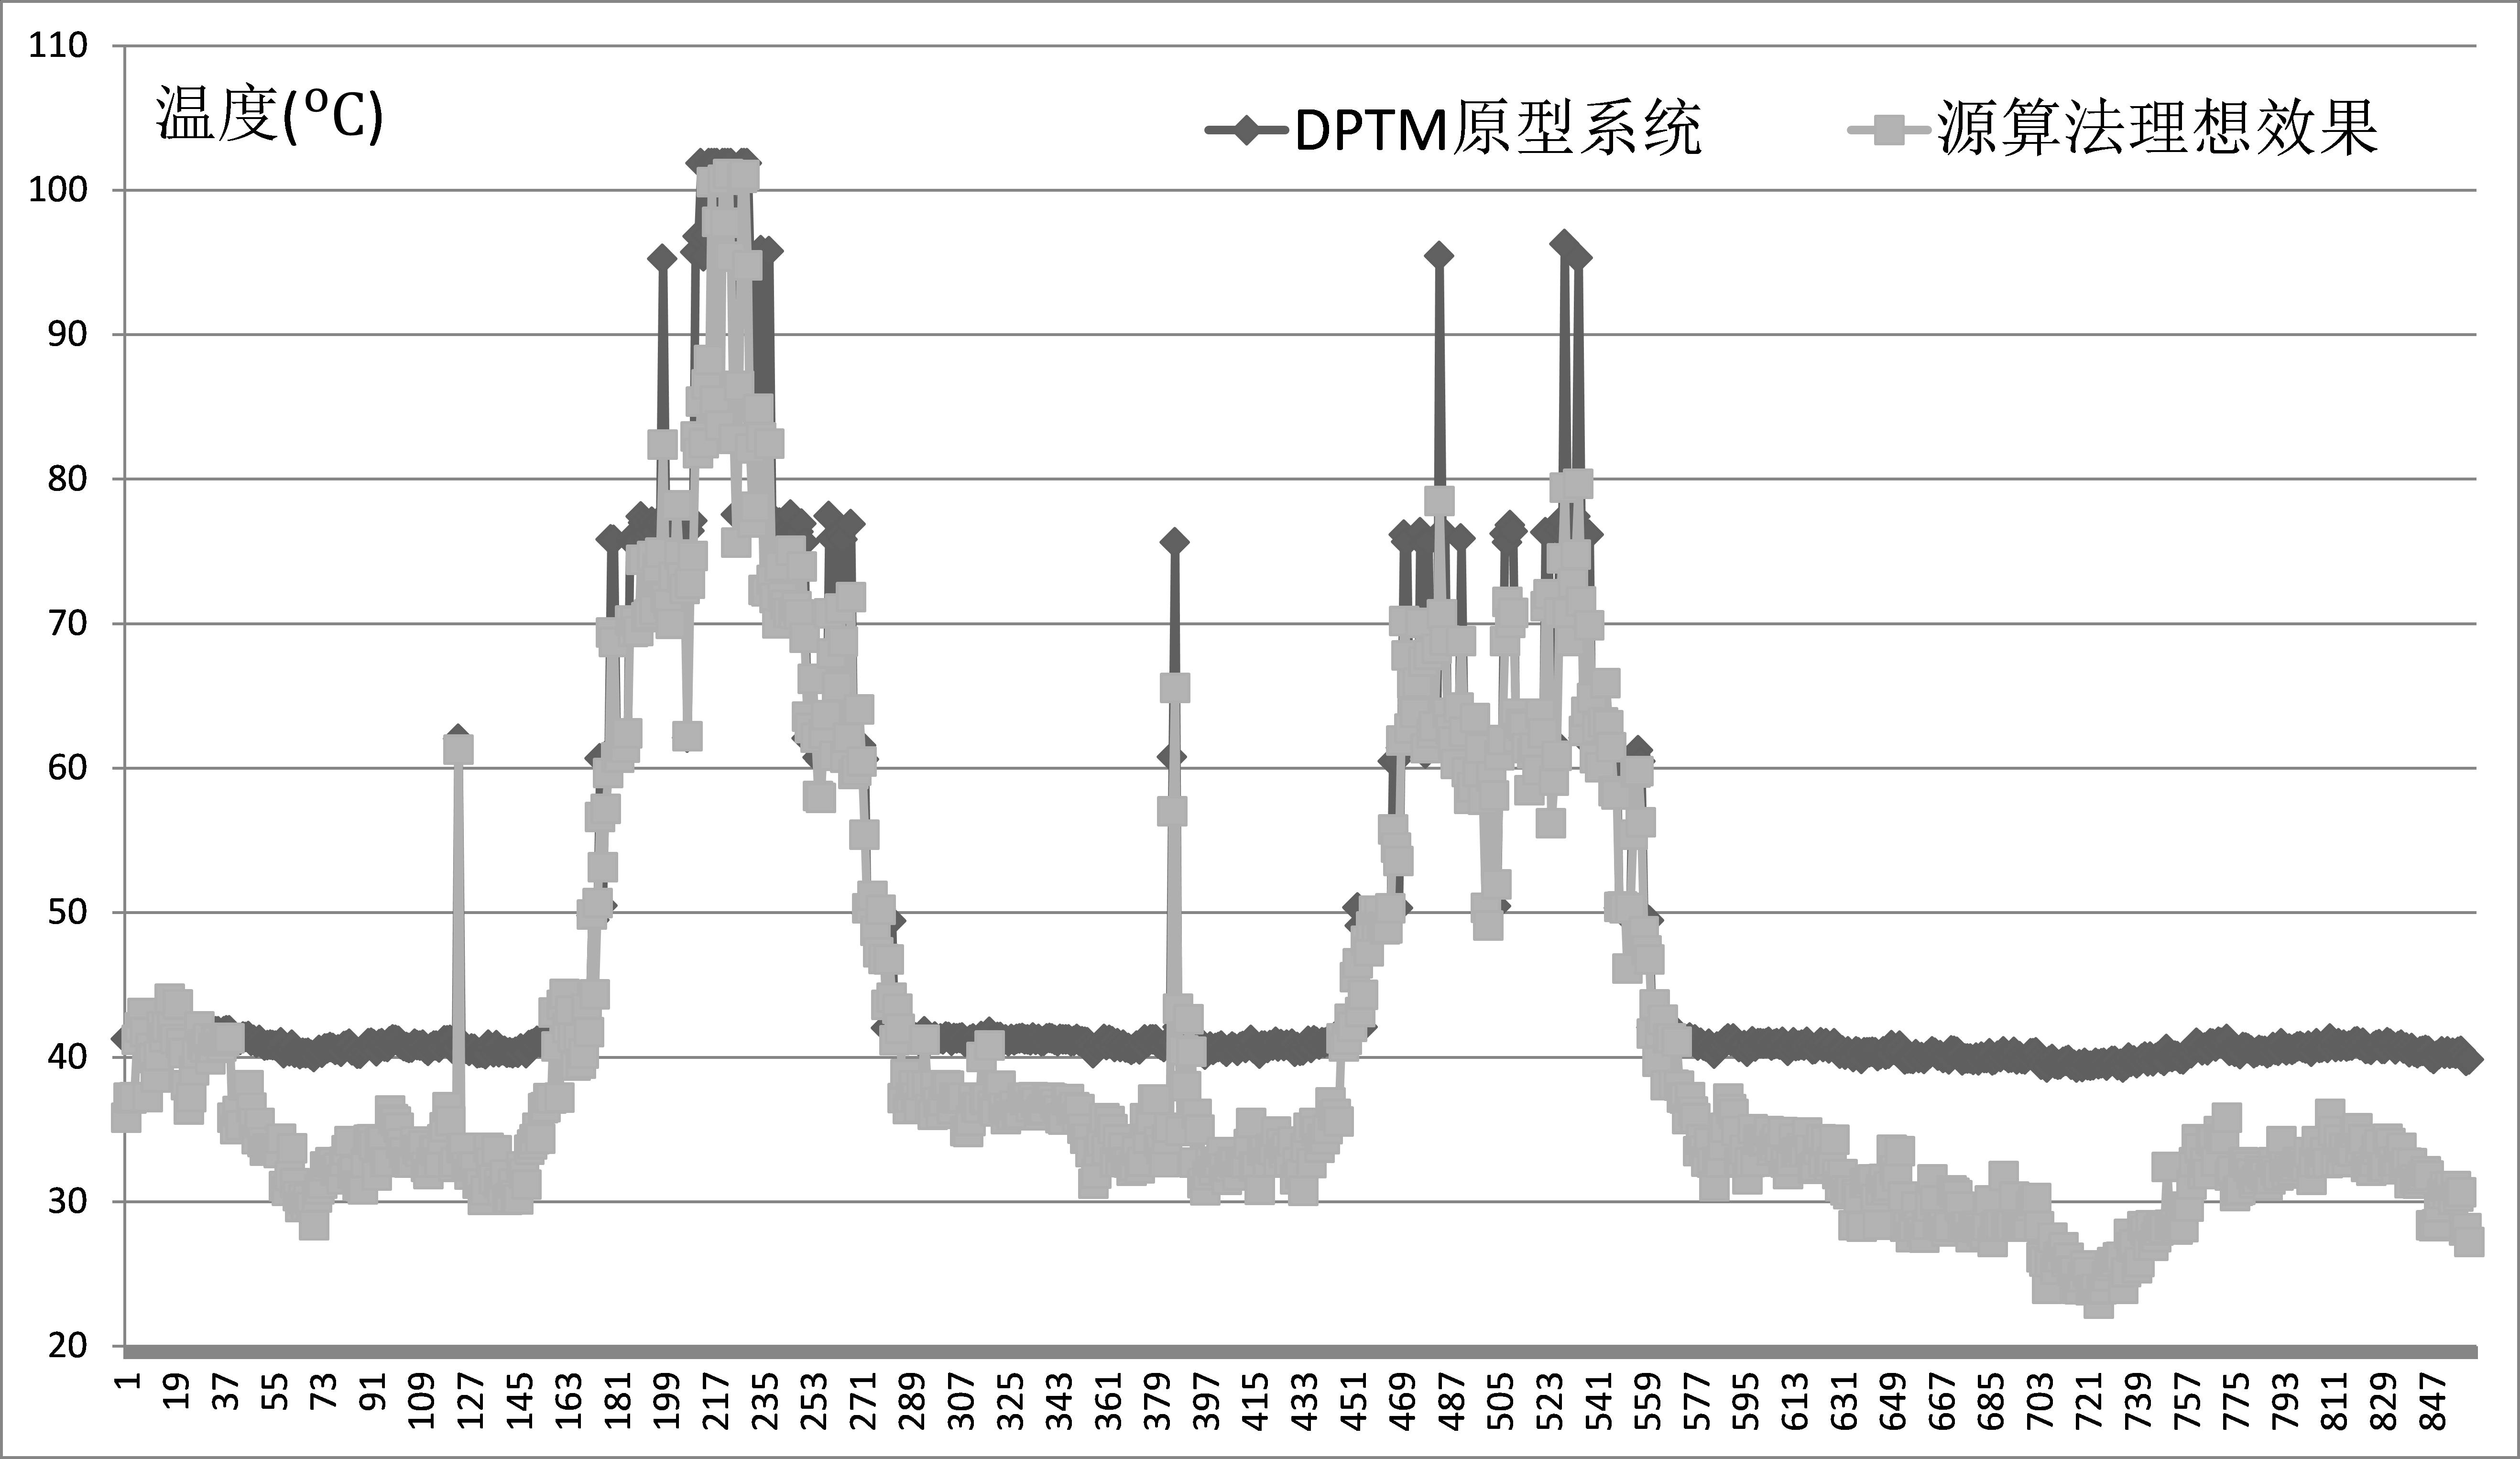
\includegraphics[width=1.0\textwidth,height=0.4\textheight]{DPTM-IDEAL-TEMP-CMP}
  \caption{DPTM原型系统VS理想效果(峰值温度)}
  \label{fig:dptm-ideal-temp-cmp}
\end{figure}

其次,同样基于\onlinecite{DPTMbyYJQ}中所得到的每个时刻工作负载真实值,采用四种源算法,分别算出每个时刻的能耗值与峰值温度, 取其中的最优值作为DPTM调度的理想值; 然后使用这批理想值来客观评价集成了TALK、PB、MO以及VP-TALK算法的DPTM原型系统的调度效果; 最后使用图\ref{fig:dptm-ideal-power-cmp}与图\ref{fig:dptm-ideal-temp-cmp}分别 比较了本文原型系统与四种对比源算法理论最优调度效果的能耗(单位$J$)和峰值温度(单位$\celsius$)。
从图\ref{fig:dptm-source-alg-power-cmp}与图\ref{fig:dptm-source-alg-temp-cmp}可以直观地看出: 与四种源算法平均调度效果相比, 本文原型系统择优式的组合DPTM算法可以明显拉低实时系统的运行能耗曲线和峰值温度曲线, 这表明对比于四种DPTM源算法,本文基于机器学习的DPTM原型系统获得了"取其长、去其短"的优化效果。 同时从表3的比较数据可以得出"本文原型系统可以获得近似最优的调度效果"的结论,其实验依据如下:
(1)与四种DPTM源算法的平均效果相比(图\ref{fig:dptm-source-alg-power-cmp}), 本文原型系统采用的择优式组合DPTM算法可获得更优的能耗优化效果, 所有时间采样点能耗的累加值$E_{TOTAL}$(总能耗)可获得18.39\%的改进, 所有时间采样点中的最大值$E_{MAX}$(最大能耗)可获得18.77\%的改进。整体改进效果非常明显。
(2)与四种DPTM源算法相比(图\ref{fig:dptm-source-alg-temp-cmp}),本文原型系统可以获得更优的峰值温度优化效果, 所有时间采样点中的最大峰值温度$T_{PMAX}$是最优, 所有时间采样点峰值温度的平均值$T_{PAVG}$是比算法均值稍弱。与四种DPTM源算法调度效果平均值相比, 本文原型系统可以获得$T_{PMAX}$1.81$\celsius$的改进,但$T_{PAVG}$ 有-1.31$\celsius$的退化。从拉低最大峰值温度的角度来讲,改进效果较为明显。
(3)通过图\ref{fig:dptm-ideal-power-cmp}与图\ref{fig:dptm-ideal-temp-cmp} 对本文原型系统的调度效果与理想值进行的直观比较, 看出本文原型系统可以获得比四种源算法均值更接近于理想值的优化效果。 与表3中理想值的$E_{TOTAL}/E_{MAX}/T_{PAVG}/T_{PMAX}$参数相比, 四种DPTM源算法调度效果平均值会产生28.64\%/30.09\%/7.71$\celsius$/9.73$\celsius$的差距, 而本文原型系统只产生了12.55\%/13.93\%/9.02$\celsius$/7.91$\celsius$差距。

\section{小结}
第\ref{cha:DPTM}章深入分析与评估了已有的主流调度算法,提出了一系列调度准则和经验。 基于这些对芯片工作休眠状态调度的经验准则,我们提出一种在能耗节省方面更具优势的DPTM调度算法VP-TALK, 以此算法为基础,综合本文所提出的预测任务负载模型,构建了一个基于负载预测的DPTM系统。本章中的仿真实验表明, (1)本文的组合模型在负载预测方面胜过众多的相关模型及算法,平均误差仅为2.89\%; (2)本文所提出的VP-TALK算法在较高的工作负载率和共同的峰值温度约束下, 分别比Pattern-Based、M-Oscillating、TALK分别节能20.54\%、11.04\%、11.42\%; (3)本文所提出的综合四种源算法、基于机器学习的DPTM原型系统较为接近理想值, 与其$E_{TOTAL}/E_{MAX}/T_{PAVG}/T_{PMAX}$参数相比, 只产生了12.55\%/13.93\%/9.02$\celsius$/7.91$\celsius$差距。 
%%% Local Variables:
%%% mode: latex
%%% TeX-master: t
%%% End:

% !Mode:: "TeX:UTF-8"

\chapter{考虑温度对漏电流功耗影响的MPSoC结构级热分析算法}
\label{cha:SSTA}


\section{多核芯片热分析的研究对象建模}
\label{sec:SSTAbasic}

\subsection{多核架构及其电热分布}

目前多核CPU普遍采用同质架构。即每个核心(core)拥有相同的逻辑功能模块(computing unit)、容量相同的专享缓存(exclusive cache),占有相同的内核面积, 同时共享最后一级缓存(last level cache,LLC)缓存、I/O等功能模块\onlinecite{TemMicroArch,TemMicArcMdlImpl}。 每个核心具有相同数量的工作模式,不同的工作模式意味着消耗不同程度的能量。一般来说,每个核心除具有一个全速高能模式外, 还具有多种耗能程度不同的节能模式\onlinecite{ThrOptTskAllocThemConstMulPro}。
在每个核心内,逻辑功能模块具有最大的功耗密度,该功能模块对应的指令L1缓存和数据L1缓存功耗密度次之, L2缓存具有的功耗密度相较而言最小。由于注入的热量大,每个核的热点(温度最高点)出现在逻辑功能模块,所以在物理设计中, 理论上说,要将逻辑功能模块布放在散热条件好的芯片边沿处,而散热条件最差的芯片中央布放功耗密度最小的LLC,从而降低芯片的热点温度。 图\ref{fig:ev6}为Alpha 21264芯片的物理布局\onlinecite{TemMicroArch},

\begin{figure}[H]
  \centering
  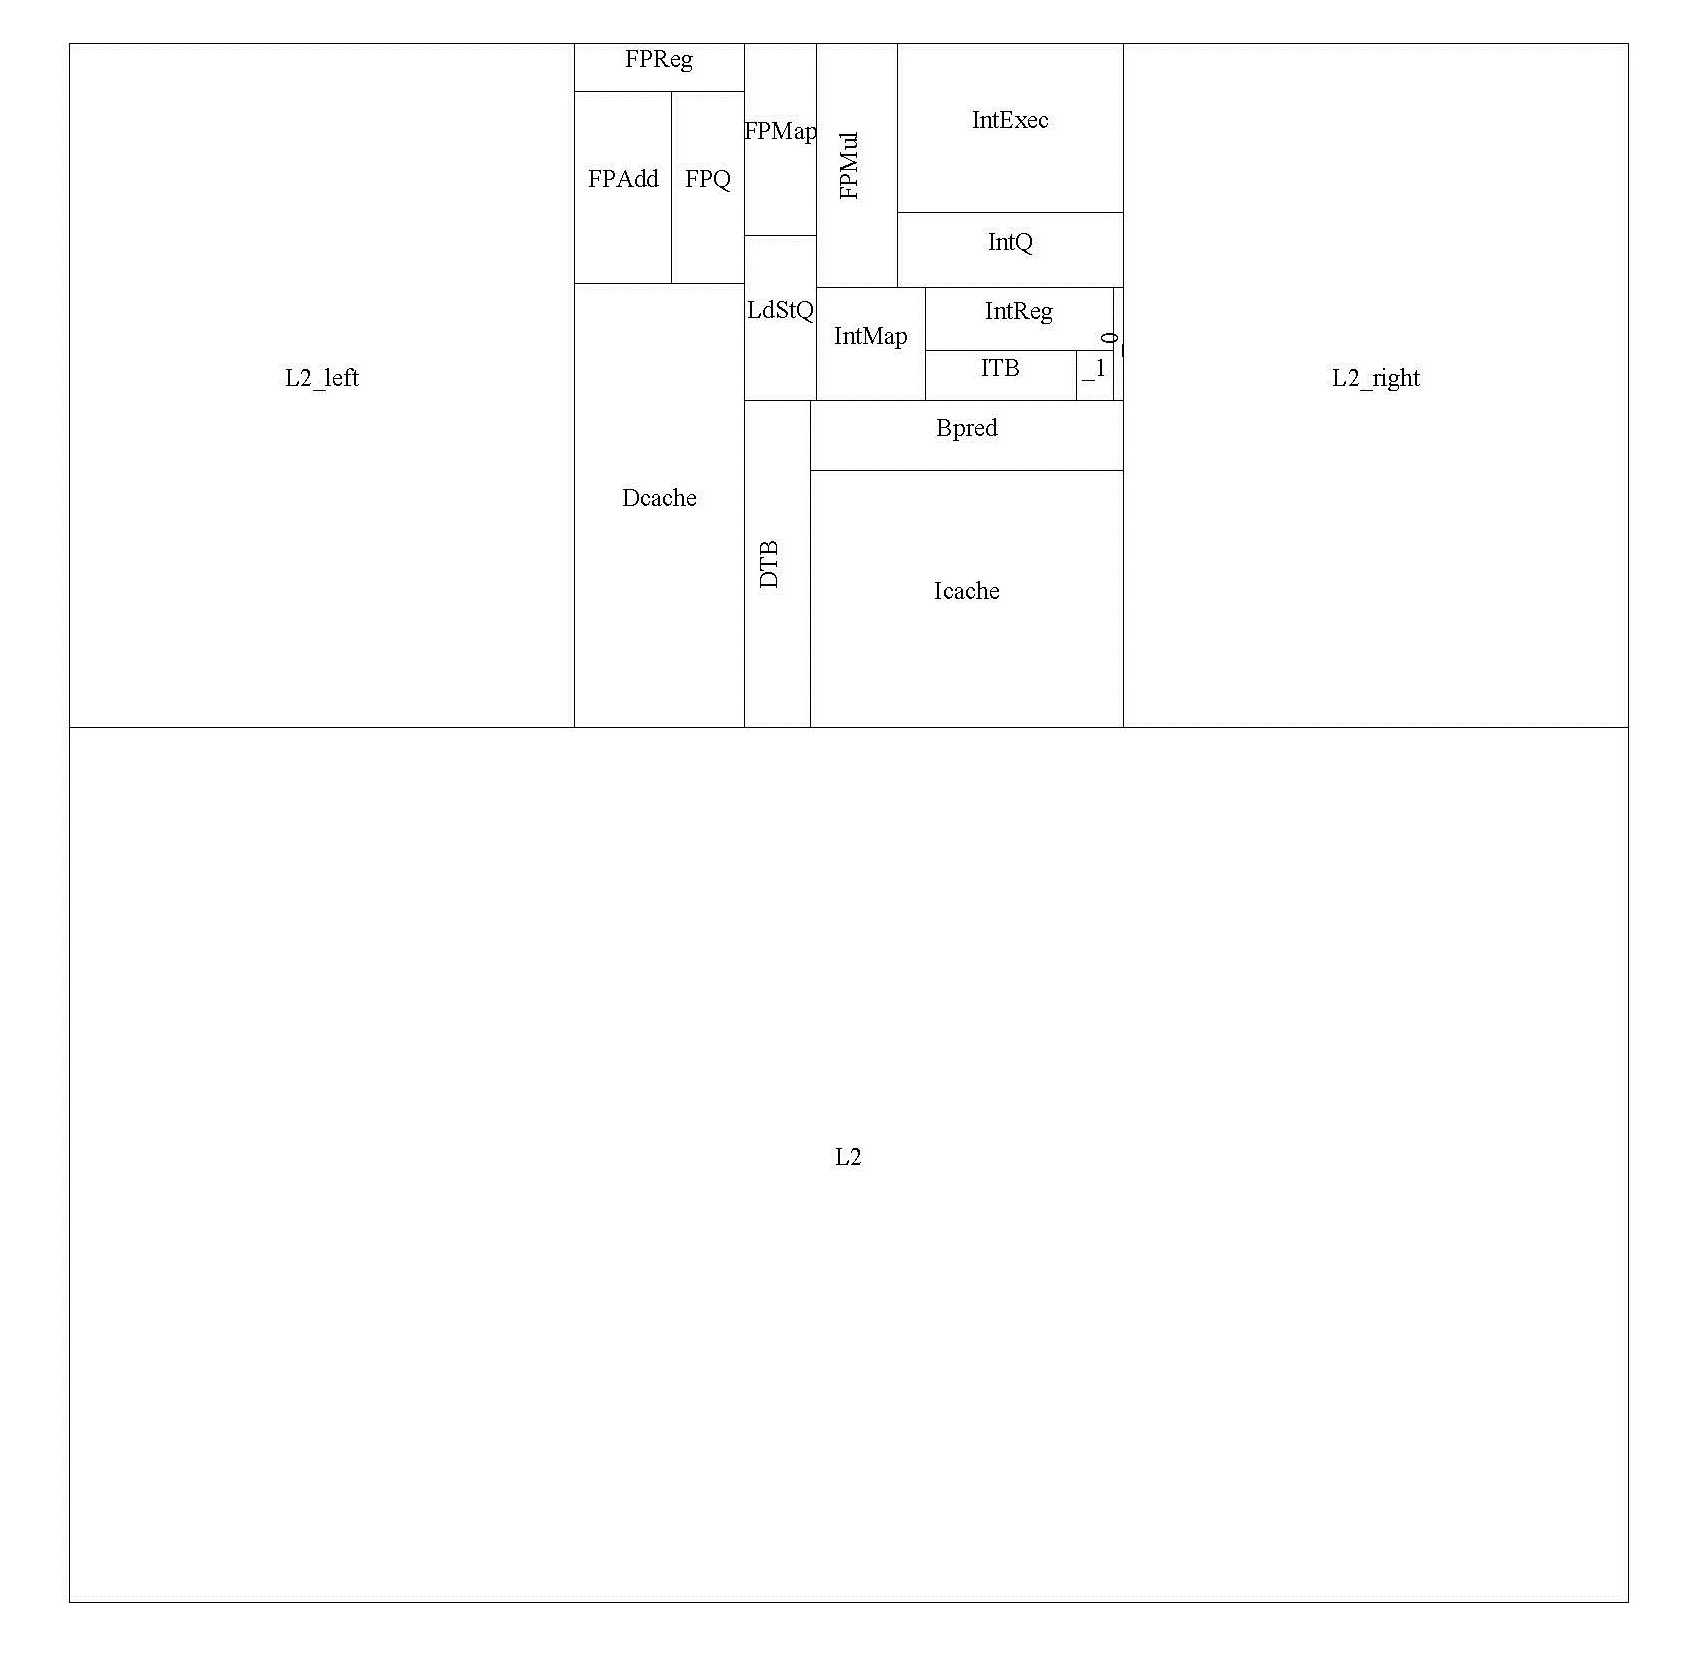
\includegraphics[width=1\textwidth,height=0.7\textheight]{EV6}
  \caption{Alpha21264芯片的物理布局}
  \label{fig:ev6}
\end{figure}


\subsection{芯片热分析及HotSpot模块级模型}

在MPSoC结构级热分析中,一般采用已有的电热等效模型,分析稳态温度分布,以降低计算复杂度[7,8]。 对于稳态热分析而言,将芯片的功耗分布作为注入的热流向量$\mathbf{P}$,对芯片的物理结构进行离散化建模后, 可以获得节点之间的热导矩阵$\mathbf{G}$, 目前多采用如下的稳态热分析方程计算节点温度分布向量$\mathbf{T}$:
\begin{equation}
\label{equ:chap4:gtp}
\mathbf{G} \times \mathbf{T} = \mathbf{P}
\end{equation}
对于多核实时功耗温度管理(dynamic power and temperature management, DPTM)研究\onlinecite{ThmBefMulCrFlrPlLimSty,TemSupVolPerfPowMdlMicroLvl}, 目前广泛采用Skadron等人提出的HotSpot热分析模型(软件)\onlinecite{TemMicroArch}构建热导矩阵$\mathbf{G}$, 并采用式\ref{equ:chap4:gtp}进行计算。 HotSpot采用基于等效热导的电路模型,将体系结构级的功能模块作为分析热点的对象。除了模块级别的热分析模型,HotSpot仍然提供了更为复杂的网格级(grid mode)热分析模型与方法。本文所指的HotSpot模型及其计算结果均指模块模式(block mode)的热分析模型与结果。 一种直观的对应芯片以及热封装的物理结构的具体建模例子如图\ref{fig:hotspot-model} 所示。电路模型在垂直热传导方向上有3层:内核(die)层、扩热(heat spreader)层、与散热片(heatsink)层,另外加入第4层热对流(heat convector)层,即与环境温度的接口。内核层根据芯片的几何布局被分为块;扩热层分为5块: 与内核层完好对应的$R_sp$以及4块呈梯形状的环绕块;散热片层按照与扩热层相似的划分方法,分为$R_hs$以及4个环绕块; 最后,从热封装到外界环境的热对流层由$R_convection$表示\onlinecite{ThrOptTskAllocThemConstMulPro,MySSTAPaper}。 层与层之间模型刻画由内核直至封装及外界环境的热流; 层内水平模型刻画相邻模块间的热扩散。内核层产生的功耗等效为每个模块中心的电流源\onlinecite{TemMicArcMdlImpl,MySSTAPaper}。 建模完成后,通过电路分析可得到芯片的温度分布。 用HotSpot计算分析Alpha 21264芯片的温度分布如图\ref{fig:ev6-grid-temp-surf}所示。

\begin{figure}[H]
  \centering
  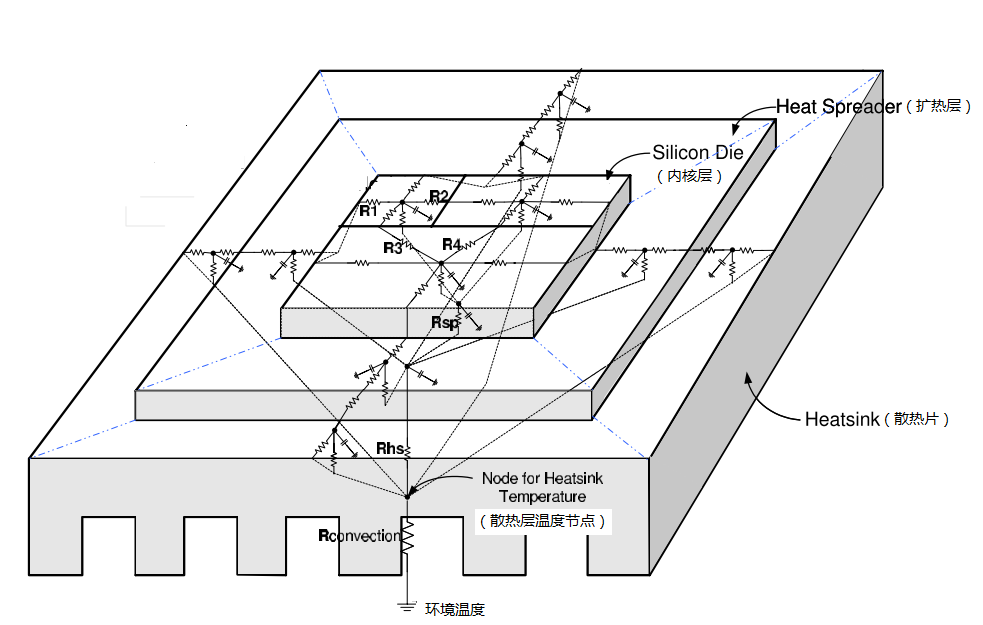
\includegraphics[width=1\textwidth,height=0.45\textheight]{HOTSPOT-MODEL}
  \caption{HotSpot对芯片的电路等效热分析模型}
  \label{fig:hotspot-model}
\end{figure}

\begin{figure}[H]
  \centering
  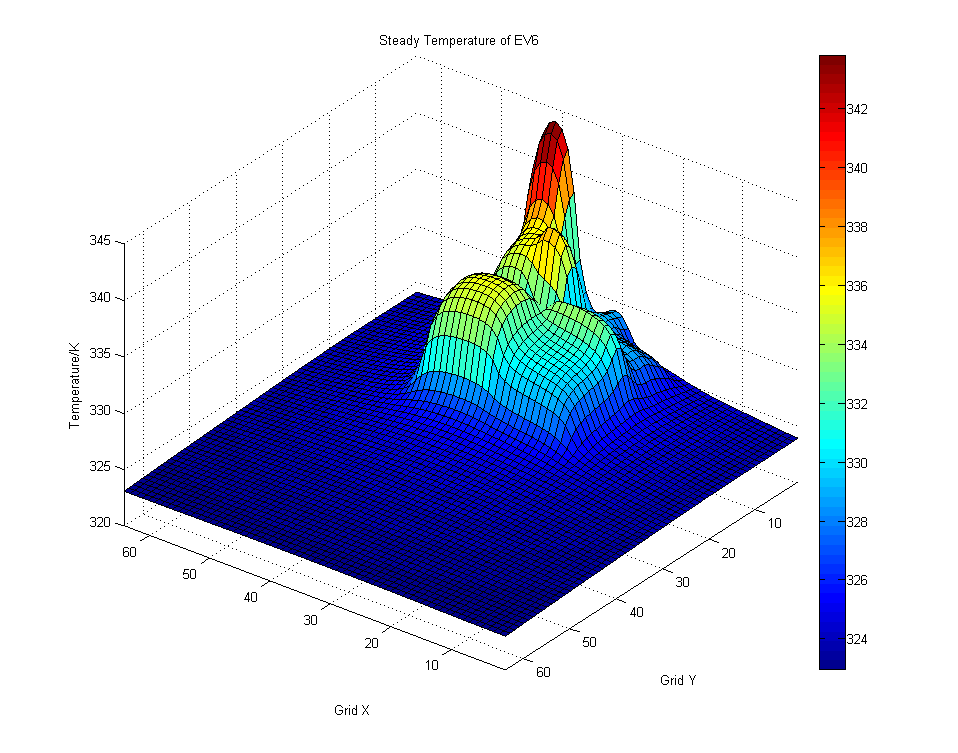
\includegraphics[width=1\textwidth,height=0.6\textheight]{EV6-GRID-TEM-SURF}
  \caption{Alpha21264芯片的温度分布}
  \label{fig:ev6-grid-temp-surf}
\end{figure}


\subsection{电热耦合效应:温度对漏电流功耗的影响}
正如\ref{sec:power}节中,式\ref{equ:chap2:active-power-simplified}、式\ref{equ:chap2:leakage-power} 所定性与定量地描述那样,芯片功耗由动态功耗$P_{dynamic}$与静态功耗$P_{leakage}$两部分组成, 随着芯片制作工艺的提高,$P_{leakage}$已成为芯片功耗的主要贡献者。 而工作温度$T$的升高可以明显增大$P_{leakage}$。这就是所谓的芯片内部电热耦合效应。在考虑电热耦合效应的热分析过程中, 需要对$T-P$采用迭代方法计算,如\ref{fig:tp-iteration}所示,对于一个16核CPU的测例(具体的实验参数设置见第\ref{cha:SSTAexperiments}章), 采用迭代算法来逼近最终的精确解。

与不考虑电热耦合效应的初始解相比,芯片最高温度与静态功耗都有了明显的增加, 这表明在芯片的温度分析中、必须考虑温度对静态功耗的影响,否则,将会产生较大的分析误差。同时,与不考虑电热耦合效应的温度分析算法相比, 由于考虑电热耦合效应的温度分析算法需要采用7次迭代计算才能获得精确解, 所以其算法复杂度是对比算法的7倍;因此降低考虑电热耦合效应的温度分析算法复杂度就具有非常重要的研究意义。
\begin{figure}[H]
  \centering
  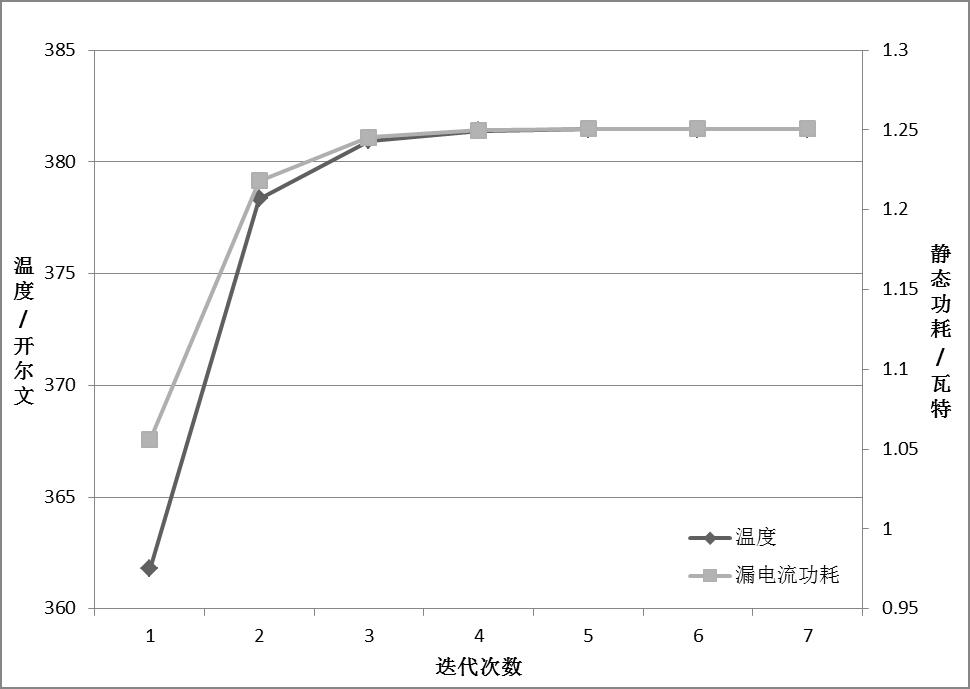
\includegraphics[width=1\textwidth,height=0.6\textheight]{TP-ITERATION}
  \caption{考虑电热耦合效应的多核芯片最高温度与静态功耗的迭代求解}
  \label{fig:tp-iteration}
\end{figure}


\section{3种MPSoC结构级热分析算法}
\label{sec:SSTAmethod}

\subsection{模块级热分析算法(简称BlockTAM算法)}
为了对功能模块进行热分析建模,按照式\ref{fig:hotspot-model}对HotSpot的多核芯片热分析模型, 采用等效电路的方法对其进行进一步简化, 为此本文假设\onlinecite{MySSTAPaper}:每个功能模块内的功耗与温度分布是均匀的,以该模块中心点的温度作为该模块的温度, 并将功耗密度乘以面积作为该模块的功耗,加于模块中心点。
在本文工作中,将模块$u$的功耗$P_{u,u}$作为注入热源。对于多核芯片, 如果仅在模块$u$加上幅值为$P_{u,u}$的阶跃激励, 其他模块均不加激励,则可以使用HotSpot模拟器获得所有模块的温度$T_{v,u}$响应曲线。 先根据$T_{u,u}$的最终收敛值$\overline{T}_{u,u}$ 可以计算出模块$u$的等效热阻$R_{u,u}$,计算公式为\ref{equ:chap4:blotam-rii}
\begin{equation}
\label{equ:chap4:blotam-rii}
R_{u,u} = \frac{\overline{T}_{u,u}}{P_{u,u}}
\end{equation}
再根据等效热阻$R_{u,u}$以及模块$v$功耗$P_{v,v}$的阶跃激励作为单一注入热源所得到的$\overline{T}_{u,v}$, 可以采用式\ref{equ:chap4:blotam-rij}计算出反映$P_{v,v}$对模块$u$温度作用关系的等效热阻$R_{u,v}$,
\begin{equation}
\label{equ:chap4:blotam-rij}
R_{u,v} = \frac{\overline{T}_{u,v}}{P_{v,v}}
\end{equation}
最后根据所获得的参数$R_{u,u}$与$R_{u,v}$ ,可以计算$P_{v,v}$对模块$u$温度计算产生影响的等效热源$P_{u,v}$:
\begin{equation}
\label{equ:chap4:blotam-pij}
P_{u,v} = \frac{\overline{T}_{u,v}}{\overline{T}_{u,u}}P_{u,u} = \frac{R_{u,v}\times P_{v,v}}{R_{u,u}\times P_{u,u}}P_{u,u}=\frac{R_{u,v}}{R_{u,u}}P_{v,v}
\end{equation}
因此,按照图\ref{fig:multicore-temp-model}中所给出的单模块温度分析模型,可以列出如下热分析表达式:
\begin{equation}
\label{equ:chap4:blotam-tii}
T_{u,u} = R_{u,u}\sum\limits_{v=1}^N P_{u,v} = R_{u,u}\widehat{P_{u}}
\end{equation}
其中$N$为多核芯片中的功能模块数目,$\widehat{P_{u}} = \sum\limits_{v=1}^N P_{u,v}$为模块$u$的等效热源,由于一个模块只有一个等效热源, 可见式\ref{equ:chap4:blotam-tii}提供的单模块热分析模型兼容了经典的单核(单模块)热分析模型\onlinecite{TemMicArcMdlImpl}。 从式\ref{equ:chap4:blotam-tii}可知:BlockTAM方法的算法时间复杂度与空间复杂度均为$O(N^2)$, 即算法复杂度为$O(N^2)$。
\begin{figure}[H]
  \centering
  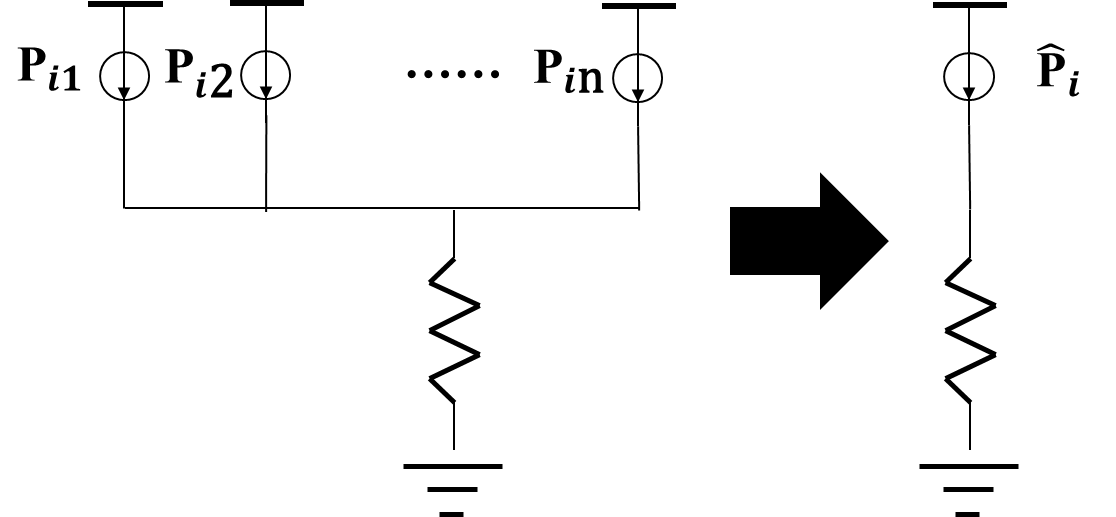
\includegraphics[width=1.0\textwidth,height=0.35\textheight]{MULTICORE-TEMP-MODEL}
  \caption{多核实时功耗温度管理的单模块与单核热分析简化等效电路模型}
  \label{fig:multicore-temp-model}
\end{figure}

\subsection{核级热分析方法(简称CoreTAM算法)}
为了对处理器核进行热分析建模,可以基于图\ref{fig:hotspot-model}中HotSpot的多核芯片热分析模型, 采用等效电路的方法对其进行进一步简化,为此,进行如下的假设\onlinecite{MySSTAPaper}:
\begin{enumerate}[1)]
\item 在处理器核多个功能模块中,逻辑模块(包括ALU等器件)产生最高的工作温度,将逻辑模块的温度作为处理器核的温度; 为了对其他核产生影响,将处理器核中所有功能模块的功耗加到逻辑模块中心。
\item 为了计算温度对漏电流功耗的影响,将逻辑模块的静-动态功耗比例、作为处理器核中所有功能模块的静-动态功耗比例, 也就是:随着工作温度的变化,变的是静-动态功耗比例,不变的是核内所有模块功耗的比例。
\end{enumerate}

基于如上假设,将核p内的所有模块均加上符合核内功耗比例要求的阶跃激励,其他核均不加激励, 则可以使用HotSpot模拟器获得所有核的温度$T_{t,s}$响应曲线。先根据$T_{s,s}$的最终收敛值$\overline{T}_{s,s}$ 可以计算出核$s$的等效热阻$R_{s,s}$,计算公式如下:
\begin{equation}
\label{equ:chap4:cortam-rpp}
R_{s,s} = \frac{\overline{T}_{s,s}}{P_{s,s}}
\end{equation}
式\ref{equ:chap4:cortam-rpp}中$P_{s,s}$是核$s$内所有模块的功耗之和。再根据等效热阻$R_{s,s}$, 以及核$t$功耗$P_{t,t}$ 的阶跃激励作为单一注入热源所得到的$\overline{T}_{s,t}$,采用如下公式计算出反映$P_{t,t}$对核$s$ 温度作用关系的等效热阻$R_{s,t}$,
\begin{equation}
\label{equ:chap4:cortam-rpq}
R_{s,t} = \frac{\overline{T}_{s,t}}{P_{t,t}}
\end{equation}
之后根据以上所获得的参数,可以计算$P_{t,t}$对核$s$温度计算产生影响的等效热源$P_{s,t}$:
\begin{equation}
\label{equ:chap4:cortam-ppq}
P_{s,t} = \frac{\overline{T}_{s,t}}{\overline{T}_{s,s}}P_{s,s} = \frac{R_{s,t}\times P_{t,t}}{R_{s,s}\times P_{s,s}}P_{s,s} = \frac{R_{s,t}}{R_{s,s}}P_{t,t}
\end{equation}
最后,按照图\ref{fig:multicore-temp-model}中所给出的热分析模型,可以列出如下热分析表达式:
\begin{equation}
\label{equ:chap4:cortam-tpp}
T_{s,s} = R_{s,s}\sum\limits_{t=1}^n P_{s,t}
\end{equation}

式\ref{equ:chap4:cortam-tpp}中$n$为多核芯片中的核数。从式\ref{equ:chap4:cortam-tpp}可知: CoreTAM方法的算法复杂度为$O(n^2)$。 从计算机系统结构可知, 核数$n$远小于模块数$N$,因此,多核芯片的核级温度分析复杂度要远小于模块级。

\subsection{考虑核内模块相互影响的改良核级热分析方法(简称BlockInsideCoreTAM算法)}
在核级热分析方法研究中,假设了核内各个模块对核内逻辑模块中心温度具有相同的相关热阻, 并且每个核内仅需计算一个点的温度;核内各模块均使用该温度来刷新模块的漏电流功耗, 会使整个核的漏电流功耗增大。为了使漏电流计算更为精确,必须计算出各自模块的温度,为此, 下面给出一个考虑核内模块相互影响的改良核级热分析方法:BlockInsideCoreTAM。在BlockInsideCoreTAM方法中,先进行如下的假设\onlinecite{MySSTAPaper}:
\begin{enumerate}[1)]
\item 核$t$的功耗$P_{t,t}$对核$s$内所有模块均产生相同的等效热量影响为$P_{s,t} = \frac{R_{s,t}}{R_{s,s}}P_{t,t}$,其中$R_{s,t}$为两个核内所有模块之间相关热阻的平均值,即
\begin{equation}
\label{equ:chap4:bicortam-rpq}
R_{s,t} = \frac{1}{m^2}\sum\limits_{u \in BS_s}\sum\limits_{v \in BS_t}R_{u,v}
\end{equation}
式\ref{equ:chap4:bicortam-rpq}中$BS_x$是核$x$内所有模块的集合。
\item 在核$s$内,模块$v$对模块$u$的等效热量影响为$P_{u,v} = \frac{R_{u,v}}{R_{u,u}}P_{v,v}$,式中$u,v \in BS_s$。
\end{enumerate}
按照以上假设,可以列出如下BlockInsideCoreTAM表达式:
\begin{equation}
\label{equ:chap4:bicortam-tii}
\frac{T_{u,u}}{R_{u,u}} = \sum\limits_{t=1,t\neq s}^n P_{s,t} + \sum\limits_{v=1}^m P_{u,v}
\end{equation}
从式\ref{equ:chap4:bicortam-tii}可知:BlockInsideCoreTAM方法的算法复杂度为$O(n^2+(m^2-1)n)$。 BlockInsideCoreTAM的计算复杂度介于CoreTAM和BlockTAM之间,当$m \ll n$时,BlockInsideCoreTAM的算法复杂度近似等于CoreTAM。




%%% 其它部分
%\backmatter

%
% % 参考文献
 \bibliographystyle{bnubib}
 \bibliography{ref/refs}

% 附录
\begin{appendix}
% !Mode:: "TeX:UTF-8"
%%% Local Variables:
%%% mode: latex
%%% TeX-master: "../main"
%%% End:

\chapter{外文资料原文}
\label{cha:engorg}
As one of the most widely used techniques in operations research, {\em
  mathematical programming} is defined as a means of maximizing a quantity known
as {\em objective function}, subject to a set of constraints represented by
equations and inequalities. Some known subtopics of mathematical programming are
linear programming, nonlinear programming, multiobjective programming, goal
programming, dynamic programming, and multilevel programming$^{[1]}$.

It is impossible to cover in a single chapter every concept of mathematical
programming. This chapter introduces only the basic concepts and techniques of
mathematical programming such that readers gain an understanding of them
throughout the book$^{[2,3]}$.


\section{Single-Objective Programming}
The general form of single-objective programming (SOP) is written
as follows,
\begin{equation}\tag*{(123)} % 如果附录中的公式不想让它出现在公式索引中,那就请
                             % 用 \tag*{xxxx}
\left\{\begin{array}{l}
\max \,\,f(x)\\[0.1 cm]
\mbox{subject to:} \\ [0.1 cm]
\qquad g_j(x)\le 0,\quad j=1,2,\cdots,p
\end{array}\right.
\end{equation}
which maximizes a real-valued function $f$ of
$x=(x_1,x_2,\cdots,x_n)$ subject to a set of constraints.

\newtheorem{mpdef}{Definition}[chapter]
\begin{mpdef}
In SOP, we call $x$ a decision vector, and
$x_1,x_2,\cdots,x_n$ decision variables. The function
$f$ is called the objective function. The set
\begin{equation}\tag*{(456)} % 这里同理,其它不再一一指定。
S=\left\{x\in\Re^n\bigm|g_j(x)\le 0,\,j=1,2,\cdots,p\right\}
\end{equation}
is called the feasible set. An element $x$ in $S$ is called a
feasible solution.
\end{mpdef}

\newtheorem{mpdefop}[mpdef]{Definition}
\begin{mpdefop}
A feasible solution $x^*$ is called the optimal
solution of SOP if and only if
\begin{equation}
f(x^*)\ge f(x)
\end{equation}
for any feasible solution $x$.
\end{mpdefop}

One of the outstanding contributions to mathematical programming was known as
the Kuhn-Tucker conditions\ref{eq:ktc}. In order to introduce them, let us give
some definitions. An inequality constraint $g_j(x)\le 0$ is said to be active at
a point $x^*$ if $g_j(x^*)=0$. A point $x^*$ satisfying $g_j(x^*)\le 0$ is said
to be regular if the gradient vectors $\nabla g_j(x)$ of all active constraints
are linearly independent.

Let $x^*$ be a regular point of the constraints of SOP and assume that all the
functions $f(x)$ and $g_j(x),j=1,2,\cdots,p$ are differentiable. If $x^*$ is a
local optimal solution, then there exist Lagrange multipliers
$\lambda_j,j=1,2,\cdots,p$ such that the following Kuhn-Tucker conditions hold,
\begin{equation}
\label{eq:ktc}
\left\{\begin{array}{l}
    \nabla f(x^*)-\sum\limits_{j=1}^p\lambda_j\nabla g_j(x^*)=0\\[0.3cm]
    \lambda_jg_j(x^*)=0,\quad j=1,2,\cdots,p\\[0.2cm]
    \lambda_j\ge 0,\quad j=1,2,\cdots,p.
\end{array}\right.
\end{equation}
If all the functions $f(x)$ and $g_j(x),j=1,2,\cdots,p$ are convex and
differentiable, and the point $x^*$ satisfies the Kuhn-Tucker conditions
(\ref{eq:ktc}), then it has been proved that the point $x^*$ is a global optimal
solution of SOP.

\subsection{Linear Programming}
\label{sec:lp}

If the functions $f(x),g_j(x),j=1,2,\cdots,p$ are all linear, then SOP is called
a {\em linear programming}.

The feasible set of linear is always convex. A point $x$ is called an extreme
point of convex set $S$ if $x\in S$ and $x$ cannot be expressed as a convex
combination of two points in $S$. It has been shown that the optimal solution to
linear programming corresponds to an extreme point of its feasible set provided
that the feasible set $S$ is bounded. This fact is the basis of the {\em simplex
  algorithm} which was developed by Dantzig as a very efficient method for
solving linear programming.
\begin{table}[ht]
\centering
  \centering
  \caption*{Table~1\hskip1em This is an example for manually numbered table, which would not appear in the list of tables}
  \label{tab:badtabular2}
  \begin{tabular}[c]{|c|m{0.8in}|c|c|c|c|c|}\hline
    \multicolumn{2}{|c|}{Network Topology} & \# of nodes &
    \multicolumn{3}{c|}{\# of clients} & Server \\\hline
    GT-ITM & Waxman Transit-Stub & 600 &
    \multirow{2}{2em}{2\%}&
    \multirow{2}{2em}{10\%}&
    \multirow{2}{2em}{50\%}&
    \multirow{2}{1.2in}{Max. Connectivity}\\\cline{1-3}
    \multicolumn{2}{|c|}{Inet-2.1} & 6000 & & & &\\\hline
    \multirow{2}{1in}{Xue} & Rui  & Ni &\multicolumn{4}{c|}{\multirow{2}*{\bnuthesis}}\\\cline{2-3}
    & \multicolumn{2}{c|}{ABCDEF} &\multicolumn{4}{c|}{} \\\hline
\end{tabular}
\end{table}

Roughly speaking, the simplex algorithm examines only the extreme points of the
feasible set, rather than all feasible points. At first, the simplex algorithm
selects an extreme point as the initial point. The successive extreme point is
selected so as to improve the objective function value. The procedure is
repeated until no improvement in objective function value can be made. The last
extreme point is the optimal solution.

\subsection{Nonlinear Programming}

If at least one of the functions $f(x),g_j(x),j=1,2,\cdots,p$ is nonlinear, then
SOP is called a {\em nonlinear programming}.

A large number of classical optimization methods have been developed to treat
special-structural nonlinear programming based on the mathematical theory
concerned with analyzing the structure of problems.

Now we consider a nonlinear programming which is confronted solely with
maximizing a real-valued function with domain $\Re^n$.  Whether derivatives are
available or not, the usual strategy is first to select a point in $\Re^n$ which
is thought to be the most likely place where the maximum exists. If there is no
information available on which to base such a selection, a point is chosen at
random. From this first point an attempt is made to construct a sequence of
points, each of which yields an improved objective function value over its
predecessor. The next point to be added to the sequence is chosen by analyzing
the behavior of the function at the previous points. This construction continues
until some termination criterion is met. Methods based upon this strategy are
called {\em ascent methods}, which can be classified as {\em direct methods},
{\em gradient methods}, and {\em Hessian methods} according to the information
about the behavior of objective function $f$. Direct methods require only that
the function can be evaluated at each point. Gradient methods require the
evaluation of first derivatives of $f$. Hessian methods require the evaluation
of second derivatives. In fact, there is no superior method for all
problems. The efficiency of a method is very much dependent upon the objective
function.


\chapter{外文资料的调研阅读报告或书面翻译}
\section{单目标规划}
北冥有鱼,其名为鲲。鲲之大,不知其几千里也。化而为鸟,其名为鹏。鹏之背,不知其几
千里也。怒而飞,其翼若垂天之云。是鸟也,海运则将徙于南冥。南冥者,天池也。
\begin{equation}\tag*{(123)}
 p(y|\mathbf{x}) = \frac{p(\mathbf{x},y)}{p(\mathbf{x})}=
\frac{p(\mathbf{x}|y)p(y)}{p(\mathbf{x})}
\end{equation}

吾生也有涯,而知也无涯。以有涯随无涯,殆已!已而为知者,殆而已矣!为善无近名,为
恶无近刑,缘督以为经,可以保身,可以全生,可以养亲,可以尽年。

\subsection{线性规划}
庖丁为文惠君解牛,手之所触,肩之所倚,足之所履,膝之所倚,砉然响然,奏刀騞然,莫
不中音,合于桑林之舞,乃中经首之会。
\begin{table}[ht]
\centering
  \caption*{表~1\hskip1em 这是手动编号但不出现在索引中的一个表格例子}
  \label{tab:badtabular3}
  \begin{tabular}[c]{|c|m{0.8in}|c|c|c|c|c|}\hline
    \multicolumn{2}{|c|}{Network Topology} & \# of nodes &
    \multicolumn{3}{c|}{\# of clients} & Server \\\hline
    GT-ITM & Waxman Transit-Stub & 600 &
    \multirow{2}{2em}{2\%}&
    \multirow{2}{2em}{10\%}&
    \multirow{2}{2em}{50\%}&
    \multirow{2}{1.2in}{Max. Connectivity}\\\cline{1-3}
    \multicolumn{2}{|c|}{Inet-2.1} & 6000 & & & &\\\hline
    \multirow{2}{1in}{Xue} & Rui  & Ni &\multicolumn{4}{c|}{\multirow{2}*{\bnuthesis}}\\\cline{2-3}
    & \multicolumn{2}{c|}{ABCDEF} &\multicolumn{4}{c|}{} \\\hline
\end{tabular}
\end{table}

\begin{table}[ht]
\centering
  \caption{正常附录表格的例子}
  \label{tab:badtabular3}
  \begin{tabular}[c]{|c|m{0.8in}|c|c|c|c|c|}\hline
    \multicolumn{2}{|c|}{Network Topology} & \# of nodes &
    \multicolumn{3}{c|}{\# of clients} & Server \\\hline
    GT-ITM & Waxman Transit-Stub & 600 &
    \multirow{2}{2em}{2\%}&
    \multirow{2}{2em}{10\%}&
    \multirow{2}{2em}{50\%}&
    \multirow{2}{1.2in}{Max. Connectivity}\\\cline{1-3}
    \multicolumn{2}{|c|}{Inet-2.1} & 6000 & & & &\\\hline
    \multirow{2}{1in}{Xue} & Rui  & Ni &\multicolumn{4}{c|}{\multirow{2}*{\bnuthesis}}\\\cline{2-3}
    & \multicolumn{2}{c|}{ABCDEF} &\multicolumn{4}{c|}{} \\\hline
\end{tabular}
\end{table}

文惠君曰:“嘻,善哉!技盖至此乎?”庖丁释刀对曰:“臣之所好者道也,进乎技矣。始臣之
解牛之时,所见无非全牛者;三年之后,未尝见全牛也;方今之时,臣以神遇而不以目视,
官知止而神欲行。依乎天理,批大郤,导大窾,因其固然。技经肯綮之未尝,而况大坬乎!
良庖岁更刀,割也;族庖月更刀,折也;今臣之刀十九年矣,所解数千牛矣,而刀刃若新发
于硎。彼节者有间而刀刃者无厚,以无厚入有间,恢恢乎其于游刃必有余地矣。是以十九年
而刀刃若新发于硎。虽然,每至于族,吾见其难为,怵然为戒,视为止,行为迟,动刀甚微,
謋然已解,如土委地。提刀而立,为之而四顾,为之踌躇满志,善刀而藏之。”

文惠君曰:“善哉!吾闻庖丁之言,得养生焉。”


\subsection{非线性规划}
孔子与柳下季为友,柳下季之弟名曰盗跖。盗跖从卒九千人,横行天下,侵暴诸侯。穴室枢
户,驱人牛马,取人妇女。贪得忘亲,不顾父母兄弟,不祭先祖。所过之邑,大国守城,小
国入保,万民苦之。孔子谓柳下季曰:“夫为人父者,必能诏其子;为人兄者,必能教其弟。
若父不能诏其子,兄不能教其弟,则无贵父子兄弟之亲矣。今先生,世之才士也,弟为盗
跖,为天下害,而弗能教也,丘窃为先生羞之。丘请为先生往说之。”

柳下季曰:“先生言为人父者必能诏其子,为人兄者必能教其弟,若子不听父之诏,弟不受
兄之教,虽今先生之辩,将奈之何哉?且跖之为人也,心如涌泉,意如飘风,强足以距敌,
辩足以饰非。顺其心则喜,逆其心则怒,易辱人以言。先生必无往。”

孔子不听,颜回为驭,子贡为右,往见盗跖。


\chapter{其它附录}
前面两个附录主要是给本科生做例子。其它附录的内容可以放到这里,当然如果你愿意,可
以把这部分也放到独立的文件中,然后将其 \verb|\input| 到主文件中。 
\end{appendix}
%
% % 学术成果
% !Mode:: "TeX:UTF-8"
\begin{paper}
\begin{enumerate}
	

	\item Jiaqi Yan, Zuying Luo, Liang Tang:《Accurate Architecture-level Thermal Analysis Methods for MPSoC with Considering Leakage Power Dependence on Temperature》 ISQED2013: 178-183. (EI 收录,检索号:20132716473440)
	\item 闫佳琪,骆祖莹,唐亮,赵国兴:《考虑温度对漏电流功耗影响的MPSoC结构级热分析方法》 计算机辅助设计与图形学学报,2013,24(11):1767-1774 (EI源刊)
	\item 闫佳琪,骆祖莹,赵国兴:《基于任务精确预测的实时功耗温度管理》,中国图形学进展(2012)- 第十七届全国计算机辅助设计与图形学学术会议(CAD/CG`2012)暨第九届全国智能CAD与数字娱乐学术会议(CIDE`2012)论文集, 2012,7:513


  \end{enumerate}

\end{paper}


% 致谢
% !Mode:: "TeX:UTF-8"
%%% Local Variables:
%%% mode: latex
%%% TeX-master: "../main"
%%% End:

\begin{ack}
人生无根蒂,飘如陌上尘。

分散随风转,此已非常身。

落地为兄弟,何必骨肉亲。

得欢当作乐,斗酒聚比邻。

盛年不重来,一日难再晨。

及时当勉励,岁月不待人。


首次接触陶渊明的这首杂诗,还是在14年前的书法课上,徐伟老师每节课一句地教授我们如何誊写。转眼十年过去, 我曾在首都博物馆与徐老师有过一面之缘,那时,徐老师已经是北京书画艺研会副会长,并兼管首都博物馆的陈列展览事宜,而我也就要本科毕业, 并决定继续留校读研究生。徐老师早已认不出我这个并非正规的书法弟子,我也只能尴尬地寒暄了几句。想想确实是“人生无根蒂,破如陌上尘”。

紧接着便是研究生入学后结识一些新面孔,当然由于各种原因,本科时很多不太熟悉的旧面孔成了每天更为亲近的面孔。 前者的一个典型例子就是沉迷游戏、并最终会靠游戏发家致富的严智同学; 后者的典型例子就是与我通一个导师的唐亮同学和最后不是和我一个导师的张儒少同学。我们四个人组成了601寝室。 每日在学习与科研之余,可以熄灯泡脚夜聊,可以香蕉甜橙西瓜,可以啤酒炸鸡英超,可以泡面火锅日昌, 真所谓“落地为兄弟,何必骨肉亲。得欢当作乐,斗酒聚比邻”。

转眼间,研究生生涯行将结束,也确实每天劳苦奋战,也确实让身体和身材都大不如前,白发多了,肚子圆了。 虽然也能在简历里写入些许学术成果,但是仍然不免感叹光阴荏苒, 还有很多事情可以做、很多事情值得做,而这些事情却来不及在这三年里触及。也正应了这最后两句诗: “盛年不重来,一日难再晨。及时当勉励,岁月不待人”。

在此,我要感谢这些在我的研究生生涯里给予了我无限鼓励、帮助的人:

感谢我的父母。虽然我的母亲由于历史原因只能完成高中,但是她却有着胜过学历的人生智慧。她的人生虽然经历了很多困难挫折, 她的身心也承受着很多痛苦,但是她却没有让我以一种消极的态度对待人生,反而用自己的行动告诉了我应该乐观豁达的对待生活, 并且鼓励我自己闯出一番事业,不像很多同龄人一样虚度青春。我也要感谢我的父亲。 纵使在很多人看来,他并不是一个值得称赞的人,但是没有他每天的辛勤工作,没有他的供养,我的求学之路也许早已经结束。 总之,没有我的父母对我学习上的支持与生活上的关爱,我绝不可能做出今天的研究成果。

感谢我的研究生导师骆祖莹副教授。骆老师为人宽厚和蔼,却又很懂得激励我们在科研上投入足够的时间与精力。 我研究生的所有成果都是在骆老师的指导下完成的,并且骆老师因为我需要出国的原因,把所有的论文第一作者的位置都让给了我。 其实多数的想法都是源自于骆老师,最后完整的idea和实现是我和骆老师无数次的交谈、讨论和验证中实现的。感谢在我一筹莫展的时候, 骆老师能为我的科研之路指明方向。在我需要一个科研伙伴时,我永远能够找到骆老师,我相信, 国内太多的研究生导师都没有骆老师一半地对学生认真负责。

感谢同实验组的赵国兴老师。赵老师是我们组内不可多得的人才,可谓十八般武器样样精通。 他扎实的数学功底,严谨的逻辑推理思维,让我们在耳濡目染下,获得了许多科研上的意外收获。 更难得的是,赵老师经常和我们打成一片,探讨各种工程与科学问题:小到软件破解、硬件升级,大到社会现状、人生感悟, 而且往往是边聊边请我们吃了一顿大餐。三年下来,欠下了赵老师无数顿饭钱,在此不知如何感谢。

感谢以周等号先生和翁先生为主的小伙伴们,因为他们组织的餐饮歌咏活动、室外运动项目都极大地丰富了学业科研之余的周末休闲时光。 特别要感谢周等号先生赠送的麦当劳可口可乐杯:我经常用它冲咖啡、绿茶、奶茶等,这些都是我工作之时无法缺少的伴侣。

感谢高性能计算实验组曾经与现在的同学,他们是杨旭、黄琨、唐亮、李晓怡、王红蕊、王嘉琪、邹甜、唐传高等同学。 特别感谢我的研究伙伴唐亮,三年来我同他一起在实验室奋斗或者打游戏。感谢杨旭与黄琨师兄在我刚进实验室之后对我的照顾。 感谢李晓怡与王红蕊为我们报销。感谢邹甜经常能找到好地方为我们改善伙食。有他们陪伴的研究生三年是我一生中最珍贵的时光。

感谢虚拟现实实验室主任与信息科学与技术学院院长周明全教授。周老师虽然每日忙于各种项目事宜,但在每个学生需要他的时候, 却并没有任何院长的架子,总是慷慨地给予帮助。感谢虚拟现实实验室的全体老师和同学们平日里的的帮助和支持!

此外,感谢北京师范大学天文系的余恒老师,虽然他并不认识我,但是一定有很多像我一样的人会由衷的感谢他的工作: 因为他制作维护的北京师范大学学位论文模板极大的方便了\LaTeX{}用户的论文写作。

本人在研究生期间的所有工作都承蒙国家自然科学基金资助,特此致谢。
\end{ack}


\end{document}
